\documentclass[a4paper,14pt]{article}
\usepackage[a4paper, mag=1000, left=2.5cm, right=1cm, top=2cm, bottom=2cm, headsep=0.7cm, footskip=1cm]{geometry}
\usepackage[utf8]{inputenc}
\usepackage[T2A]{fontenc}
\usepackage[english,russian]{babel}
\usepackage{indentfirst}
%\usepackage[dvipsnames]{xcolor}
\usepackage[colorlinks]{hyperref}
\usepackage{amsfonts} 
\usepackage{amsmath}
\usepackage{graphicx}
\usepackage{float}

\DeclareGraphicsExtensions{.png,.jpg}

\usepackage{fancyhdr}
\pagestyle{fancy}
\fancyhead[LE,RO]{\thepage}
\fancyfoot{}

\usepackage{listings}

\hypersetup{linkcolor=black}

\title{non-linear equations}
\author{Иван Золин}
\date{2023}
\thispagestyle{empty}
\begin{document}
	
	\begin{titlepage}
		\begin{center}
			\textsc{
				Санкт-Петербургский политехнический университет имени Петра Великого \\[5mm]
				Институт прикладной математики и механики\\[2mm]
				Высшая школа прикладной математики и физики            
			}   
			\vfill
			\textbf{\large
				Математическая статистика\\
				Отчёт по лабораторным работам №1-4 \\[3mm]
			}                
		\end{center}
		
		\vfill
		\hfill
		\begin{minipage}{0.5\textwidth}
			Выполнил: \\[2mm]   
			Студент: Золин Иван \\
			Группа: 5030102/00201\\
		\end{minipage}
		
		\hfill
		\begin{minipage}{0.5\textwidth}
			Принял: \\[2mm]
			к. ф.-м. н., доцент \\   
			Баженов Александр Николаевич
		\end{minipage}
		
		\vfill
		\begin{center}
			Санкт-Петербург \\2023 г.
		\end{center}
	\end{titlepage}
	
	\tableofcontents
	\newpage
	\listoffigures
	\newpage
	\listoftables
	\newpage
	
	\section{Постановка задачи}
	\paragraph{Для четырех распределений:}
	\begin{itemize}
		\item Нормальное распределение: $N(x, 0, 1)$
		\item Распределение Коши: $C(x, 0, 1)$
		\item Распределение Лапласа: $L(x, 0, \frac{1}{\sqrt{2}})$
		\item Распределение Пуассона: $P(k, 10)$
		\item Равномерное распределение: $U(x, -\sqrt{3}, \sqrt{3})$
	\end{itemize}
	\paragraph{Выполнить следующие задачи:}
	\begin{enumerate}
		\item Сгенерировать выборки размером 10, 50 и 1000 элементов.
		Построить на одном рисунке гистограмму и график плотности распределения.
		
		\item Сгенерировать выборки размером 10, 100 и 1000 элементов.
		Для каждой выборки вычислить следующие статистические характеристики положения данных: $\overline{x}, med x, z_R, z_Q, z_{tr}$. Повторить такие вычисления 1000 раз для каждой выборки и найти среднее характеристик положения и их квадратов:
		
		\begin{equation}
			E(z)=\overline{z}
		\end{equation}
		
		Вычислить оценку дисперсии по формуле:
		
		\begin{equation}
			D(z)=\overline{z^2}-\overline{z}^2
		\end{equation}
		
		Представить полученные данные в виде таблиц.
		
		\item Сгенерировать выборки размером 20 и 100 элементов.
		\newline Построить для них боксплот Тьюки.
		Для каждого распределения определить долю выбросов экспериментально (сгенерировав выборку, соответствующую распределению 1000
		раз, и вычислив среднюю долю выбросов) и сравнить с результатами,
		полученными теоретически.
		
		\item Сгенерировать выборки размером 20, 60 и 100 элементов.
		Построить на них эмпирические функции распределения и ядерные оценки плотности распределения на отрезке $[-4; 4]$ для непрерывных распределений и на отрезке $[6; 14]$ для распределения Пуассона.
	\end{enumerate}
	\newpage
	\section{Теория}
	\subsection{Распределения}
	Плотности классических распределений:
	
	\begin{itemize}
		\item Нормальное распределение
		
		\begin{equation}
			N(x, 0, 1) = \tfrac{1}{\sqrt{2\pi}}e^{-\frac{x^2}{2}}
		\end{equation}
		
		\item Распределение Коши
		
		\begin{equation}
			C(x, 0, 1) = \dfrac{1}{\pi}\dfrac{1}{x^2+1}
		\end{equation}
		
		\item Распределение Лапласа
		
		\begin{equation}
			L(x, 0, \frac{1}{\sqrt{2}}) =\frac{1}{\sqrt{2}}e^{-{\sqrt{2}}|x|}
		\end{equation}
		
		\item Распределение Пуассона
		
		\begin{equation}
			P(k, 10) = \tfrac{10^k}{k!}e^{-10}
		\end{equation}
		
		\item Равномерное распределение
		
		\begin{equation}
			U(x, -\sqrt{3}, \sqrt{3}) =
			\begin{cases} 
				\;\; \dfrac{1}{2\sqrt{3}} \;\;\;\; \text{при} \;\;\;\; |x| \leq \sqrt{3}\\
				\,\,\,\:\;\; 0 \;\;\;\;\;\;\; \text{при} \;\;\;\; |x| > \sqrt{3}
			\end{cases}
		\end{equation}
		
	\end{itemize}
	
	\subsubsection{Определение}
	
	Гистограмма в математической статистике --- это функция, приближающая плотность вероятности некоторого распределения, построенная на основе выборки из него \cite{s:hist}.
	
	\subsubsection{Графическое описание}
	
	Графически гистограмма строится следующим образом. Сначала множество значений, которое может принимать элемент выборки, разбивается на несколько интервалов. Чаще всего эти интервалы берут одинаковыми, но это не является строгим требованием. Эти интервалы откладываются на горизонтальной оси, затем над каждым рисуется прямоугольник. Если все интервалы были одинаковыми, то высота каждого прямоугольника пропорциональна числу элементов выборки, попадающих в соответствующий интервал. Если интервалы разные, то высота прямоугольника выбирается таким образом, чтобы его площадь была пропорциональна числу элементов выборки, которые попали в этот интервал \cite{s:hist}.
	
	\subsubsection{Использование}
	
	Гистограммы применяются в основном для визуализации данных на начальном этапе статистической обработки.\\
	Построение гистограмм используется для получения эмпирической оценки плотности распределения случайной величины. Для построения гистограммы наблюдаемый диапазон изменения случайной величины разбивается на несколько интервалов и подсчитывается доля от всех измерений, попавшая в каждый из интервалов. Величина каждой доли, отнесенная к величине интервала, принимается в качестве оценки значения плотности распределения на соответствующем интервале \cite{s:hist}.\\
	Они являются мощным инструментом для исследования неизвестных распределений.\\
	В частности, на этом построены различные способы обработки сигналов, изображений и других статистических объектов. Применение гистограмм к обработке экспериментальных данных позволяет устранять артефакты - шумы и выбросы, мешающие работе с данными и не являющиеся содержательными. \\
	Шумы определяются как горизонтальные участки сигнала. Присутствуют они только до и
	после полезного сигнала, на нем они быть не могут. Определяются участки шума так: находятся границы 2-ух самых больших столбцов гистограммы полученного сигнала, затем путем прохода по сигналу в обе стороны окном определнного размера и сравнения процентного соотношения значений внутри границ большого столбца с выбранным порогом, принимается решение о пометке участка как шумового при превышении этого порога.\\
	Выбросы —  экстремальные значения во входных данных, находящиеся далеко за пределами других наблюдений. На гистограмме выбросы будут формировать одиночные пики. Выбросы следует заменить чем-то разумным (средним, медианой в окрестности). Нужно идти по гистограмме скользящим окном (параметр), и, что вылетает далеко по гистограмме (или за 3 сигмы), заменять медианным значением. Тогда ожидается, что колонны гистограммы сравняются с пейзажем.
	
	
	\subsection{Вариационный ряд}
	
	Вариационным рядом называется последовательность элементов выборки, расположенных в неубывающем порядке. Одинаковые элементы повторяются \cite[с. 409]{b:probSectMath}.\\
	Запись вариационного ряда: $x_{(1)}, x_{(2)}, \, ... \: , x_{(n)}$.\\
	Элементы вариационного ряда $x_{(i)} \;\; (i = 1, 2, \, ... \: , n)$ называются порядковыми статистиками.
	
	\subsection{Выборочные числовые характеристики}
	
	С помощью выборки образуются её числовые характеристики. Это числовые характеристики дискретной случайной величины $X^*$, принимающей выборочные значения $x_1, x_2, \, ... \: , x_n$ \cite[с. 411]{b:probSectMath}.
	
	\subsubsection{Характеристики положения}
	
	\begin{itemize}
		\item Выборочное среднее
		
		\begin{equation} \label{eq:mean}
			\overline{x} = \tfrac{1}{n}\sum\limits_{i=1}^n x_i
		\end{equation}
		
		\item Выборочная медиана
		
		\begin{equation} \label{eq:med}
			med \: x = 
			\begin{cases} 
				\;\;\;\;\;\;\; x_{(l+1)} \:\;\;\;\;\;\;\;\;\; \text{при} \;\;\;\; n = 2l + 1\\
				\;\; \dfrac{x_{(l)} + x_{(l+1)}}{2} \;\;\;\; \text{при} \;\;\;\; n = 2l
			\end{cases}
		\end{equation}
		
		\item Полусумма экстремальных выборочных элементов
		
		\begin{equation} \label{eq:zR}
			z_R = \dfrac{x_{(1)} + x_{(n)}}{2}
		\end{equation}
		
		\item Полусумма квартилей
		
		Выборочная квартиль $z_p$ порядка $p$ определяется формулой
		
		\begin{equation}
			z_p =
			\begin{cases}
				\;\; x_{([np]+1)} \;\;\;\; \text{при} \;\; np \;\; \text{дробном},\\
				\;\;\;\;\; x_{(np)} \,\:\;\;\;\;\; \text{при} \;\; np \;\; \text{целом}.
			\end{cases}
		\end{equation}
		
		Полусумма квартилей
		
		\begin{equation} \label{eq:zQ}
			z_Q = \dfrac{z_{1/4} + z_{3/4}}{2}
		\end{equation}
		
		\item Усечённое среднее
		
		\begin{equation} \label{eq:zTr}
			z_{tr} = \tfrac{1}{n-2r}\sum\limits_{i=r+1}^{n-r} x_{(i)}, \;\;\;\; r \approx \dfrac{n}{4}
		\end{equation}
		
	\end{itemize}
	
	\subsubsection{Характеристики рассеяния}
	
	Выборочная дисперсия
	
	\begin{equation}
		D = \tfrac{1}{n}\sum\limits_{i=1}^{n} (x_i - \overline{x})^2
	\end{equation}
	
	\subsection{Боксплот Тьюки}
	
	\subsubsection{Определение}
	
	Боксплот (англ. box plot) --- график, использующийся в описательной статистике, компактно изображающий одномерное распределение вероятностей.
	
	\subsubsection{Описание}
	
	Такой вид диаграммы в удобной форме показывает медиану, нижний и верхний квартили и выбросы. Несколько таких ящиков можно нарисовать бок о бок, чтобы визуально сравнивать одно распределение с другим; их можно располагать как горизонтально, так и вертикально. Расстояния между различными частями ящика позволяют определить степень разброса (дисперсии) и асимметрии данных и выявить выбросы \cite{s:boxplot}. 
	
	\subsubsection{Построение}
	
	Границами ящика служат первый и третий квартили, линия в середине ящика --- медиана. Концы усов --- края статистически значимой выборки (без выбросов). Длину «усов» определяют разность первого квартиля и полутора межквартильных расстояний и сумма третьего квартиля и полутора межквартильных расстояний. Формула имеет вид
	
	\begin{equation} \label{eq:boundBoxplot}
		X_1 = Q_1 - \dfrac{3}{2}(Q_3 - Q_1), \;\; X_2 = Q_3 + \dfrac{3}{2}(Q_3 - Q_1),
	\end{equation}
	
	где $X_1$ --- нижняя граница уса, $X_2$ --- верхняя граница уса, $Q_1$ --- первый квартиль, $Q_3$ --- третий квартиль.
	
	Данные, выходящие за границы усов (выбросы), отображаются на графике в виде маленьких кружков \cite{s:boxplot}.
	
	\subsection{Теоретическая вероятность выбросов}
	
	Встроенными средствами языка программирования R в среде разработки RStudio можно вычислить теоретические первый и третий квартили распределений ($Q_1^\text{т}$ и $Q_3^\text{т}$ соответственно). По формуле \eqref{eq:boundBoxplot} можно вычислить теоретические нижнюю и верхнюю границы уса ($X_1^\text{т}$ и $X_2^\text{т}$ соответственно). Выбросами считаются величины $x$, такие что:
	
	\begin{equation}
		\left[ 
		\begin{gathered} 
			x < X_1^\text{т}\\ 
			x > X_2^\text{т}\\ 
		\end{gathered} 
		\right.
	\end{equation}
	
	Теоретическая вероятность выбросов для непрерывных распределений
	
	\begin{equation} \label{eq:probTheorCont}
		P_\text{в}^\text{т} = P(x < X_1^\text{т}) + P(x > X_2^\text{т}) = F(X_1^\text{т}) + \Big(1 - F(X_2^\text{т})\Big),
	\end{equation}
	
	где $F(X) = P(x \le X)$ - функция распределения.\\
	
	Теоретическая вероятность выбросов для дискретных распределений
	
	\begin{equation} \label{eq:probTheorDisc}
		P_\text{в}^\text{т} = P(x < X_1^\text{т}) + P(x > X_2^\text{т}) = \Big(F(X_1^\text{т}) - P(x = X_1^\text{т})\Big) + \Big(1 - F(X_2^\text{т})\Big),
	\end{equation}
	
	где $F(X) = P(x \le X)$ - функция распределения.
	
	\subsection{Эмпирическая функция распределения}
	
	\subsubsection{Статистический ряд}
	
	Статистическим рядом называется последовательность различных элементов выборки $z_1, z_2, \, ... \: , z_k$, расположенных в возрастающем порядке с указанием частот $n_1, n_2, \, ... \: , n_k$, с которыми эти элементы содержатся в выборке.
	
	Статистический ряд обычно записывается в виде таблицы
	
	\begin{table}[h!]
		\begin{center}
			\begin{tabular}{|c|c|c|c|c|}
				\hline
				$z$ & $z_1$ & $z_2$ & $...$ & $z_k$ \\
				\hline
				$n$ & $n_1$ & $n_2$ & $...$ & $n_k$ \\
				\hline
			\end{tabular}
		\end{center}
		\caption{Статистический ряд}
	\end{table} 
	
	\subsubsection{Определение}
	
	Эмпирической (выборочной) функцией распределения (э. ф. р.) называется относительная частота события $X < x$, полученная по данной выборке:
	
	\begin{equation}
		F_n^*(x) = P^*(X < x).
	\end{equation}
	
	\subsubsection{Описание}
	
	Для получения относительной частоты $P^*(X < x)$ просуммируем в статистическом ряде, построенном по данной выборке, все частоты $n_i$, для которых элементы $z_i$ статистического ряда меньше $x$. Тогда $P^*(X < x) = \tfrac{1}{n}\sum\limits_{z_i < x}n_i$. Получаем
	
	\begin{equation}
		F^*(x) = \tfrac{1}{n}\sum\limits_{z_i < x}n_i.
	\end{equation}
	
	$F^*(x)$ --- функция распределения дискретной случайной величины $X^*$, заданной таблицей распределения
	
	\begin{table}[h!]
		\begin{center}
			\begin{tabular}{|c|c|c|c|c|}
				\hline
				$X^*$ & $z_1$ & $z_2$ & $...$ & $z_k$ \\
				\hline
				$P$ & $\dfrac{n_1}{n}$ & $\dfrac{n_2}{n}$ & $...$ & $\dfrac{n_k}{n}$ \\
				\hline
			\end{tabular}
		\end{center}
		\caption{Таблица распределения}
	\end{table}
	
	Эмпирическая функция распределения является оценкой, т. е. приближённым значением, генеральной функции распределения
	
	\begin{equation}
		F_n^*(x) \approx F_X(x).
	\end{equation}
	
	\subsection{Оценки плотности вероятности}
	
	\subsubsection{Определение}
	
	Оценкой плотности вероятности $f(x)$ называется функция $\widehat{f}(x)$, построенная на основе выборки, приближённо равная $f(x)$
	
	\begin{equation}
		\widehat{f}(x) \approx f(x).
	\end{equation}
	
	\subsubsection{Ядерные оценки}
	
	Представим оценку в виде суммы с числом слагаемых, равным объёму выборки:
	
	\begin{equation}
		\widehat{f}_n(x) = \tfrac{1}{nh_n}\sum\limits_{i=1}^n K\left( \tfrac{x - x_i}{h_n} \right).
	\end{equation}
	
	Здесь функция $K(u)$, называемая ядерной (ядром), непрерывна и является плотностью вероятности, $x_1, \, ... \: , x_n$ --- элементы выборки, $\{h_n\}$ --- любая последовательность положительных чисел, обладающая свойствами
	
	\begin{equation}
		h_n \underset{n \to \infty}{\longrightarrow} 0; \qquad \dfrac{h_n}{n^{-1}} \underset{n \to \infty}{\longrightarrow} \infty.
	\end{equation}
	
	Такие оценки называются непрерывными ядерными \cite[с. 421-423]{b:probSectMath}.\\
	
	Замечание. Свойство, означающее сближение оценки с оцениваемой величиной при $n \rightarrow \infty$ в каком-либо смысле, называется состоятельностью оценки.\\
	
	Если плотность $f(x)$ кусочно-непрерывная, то ядерная оценка плотности является состоятельной при соблюдении условий, накладываемых на параметр сглаживания $h_n$, а также на ядро $K(u)$.\\
	
	Гауссово (нормальное) ядро \cite[с. 38]{a:nonParamRegr}
	
	\begin{equation}
		K(u) = \tfrac{1}{\sqrt{2\pi}}e^{-\tfrac{u^2}{2}}.
	\end{equation}
	
	Правило Сильвермана \cite[с. 44]{a:nonParamRegr}
	
	\begin{equation}
		h_n = 1.06\hat{\sigma}n^{-1/5},
	\end{equation}
	
	где $\hat{\sigma}$ - выборочное стандартное отклонение.
	
	\subsubsection{Оценка качества ядерных приближений}
	
	После получения результатов возникает необходимость оценить качество ядерных приближений. Приведем в пример один из приемов количественных описаний сходства кривых - метод Фреше. \\
	
	Расстояние Фреше $-$ это мера сходства кривых, принимающая во внимание число и порядок точек вдоль кривых. Расстояние названо по имени французского математика Мориса Фреше.
	Метрика Фреше принимает во внимание течение лвух кривых, посколько пары точек, расстояние между которыми определяет расстояние Фреше, <<пробегают>> вдоль кривых.
	Расстояние Фреше между двумя кривыми $-$ это не длина самого короткого поводка, с котрым можно пройти все пути, а самый короткий, при котором можно пройти этот путь. \\
	
	Определим кривую как непрерывное отображение $f: [a,b] \rightarrow V$, где $a, b \in R$ и $a \leq b$ и $(V,d) - $ метрическое пространство.
	Даны две кривые $f: [a,b] \rightarrow V$ и $g: [a',b'] \rightarrow V$, их расстояние Фреше определено в виде:
	\begin{equation}
		\delta F(f,g) = \inf_{\alpha, \beta}\max_{t \in [0,1]}{\{d(f(\alpha(t)), g(\beta(t)))\}}
	\end{equation}
	
	где $\alpha$ (соответственно $\beta$) $-$ произвольная непрерывная неубывающая функция из $[0, 1]$ на $[a, b]$ (соттветственно $[a',b']$). \\
	При вычислении расстояния Фреше между произвольными кривыми обычно аппроксимируют кривые многоугольными кривыми. Многоульная кривая $-$ это кривая $P: [0,n] \rightarrow V$, где $n - $ натуральное число, такое, что для каждого $i \in [0,n-1]$ ограничение $P$ к интервалу $[i,i+1]$ является аффинным, то есть $P(i+\lambda) = (1-\lambda)P(i)+\lambda P(i+1)$. \\
	Для заданных многоугольных кривых $P$ и $Q$ их дискретное расстояние Фреше определяется как:
	%\begin{equation}
	%\delta_{dF}(P,Q)=min\norm L \norm
	%\end{equation}
	где $L - PQ$.
	
	Необязательно решение $ - $ пара точек, между которыми найдено расстояние Фреше, $-$ является единственным. \\
	
	Рассмотрим расстояние Фреше для двух кривых: ядерной оценки плотности для равномерного распределения и самого равномерного распределения при $n=100$:
		\section{Реализация}
	\subsection{Описание}
	Данная лабораторная работа была выполнена с использованием языка
	программирования Python 3.10 в среде разработки PyCharm с
	использованием следующих библиотек:
	\begin{itemize}
		\item math - использование математических функций
		\item matplotlib версии 3.7.1 - построение графиков
		\item numpy версии 1.24.2 - использование многомерных массивов
		\item prettytable версии 3.6.0 - вывод таблиц в консоли 
		\item scipy версии 1.10.1 - статические распределения и функции
		\item seaborn версии 0.12.2 - посроение графиков, визуализация
		\item statsmodels - дополнение к scipy, использование статистических вычислений, включая описательную статистику, оценку и вывод статистических моделей
	\end{itemize}
	Отчёт подготовлен с помощью языка LaTEX в редакторе TexStudio.
		\subsection{Ссылка на репозиторий}
		\url{https://github.com/IMZolin/Math-statistics-labs} \ - GitHub репозиторий
	
	\section{Результаты}
	\subsection{Гистограмма и график плотности распределения}
	\begin{figure}[H]
		\centering
		\begin{tabular}{c c c}
			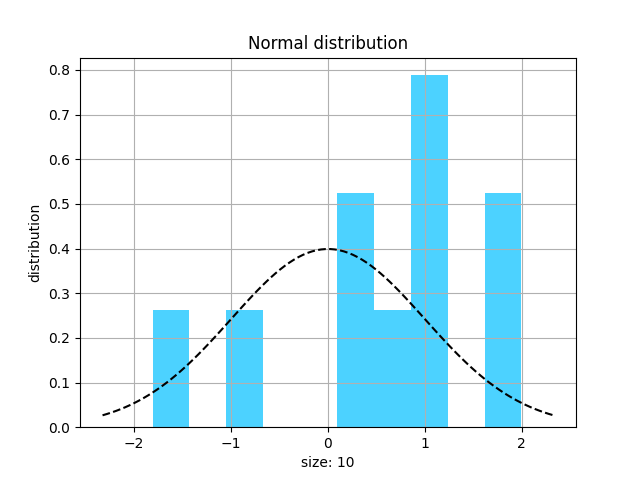
\includegraphics[height = 0.25\textheight, width = 0.31\textwidth]{../image/lab1/lab1_norm_10.png}
			& 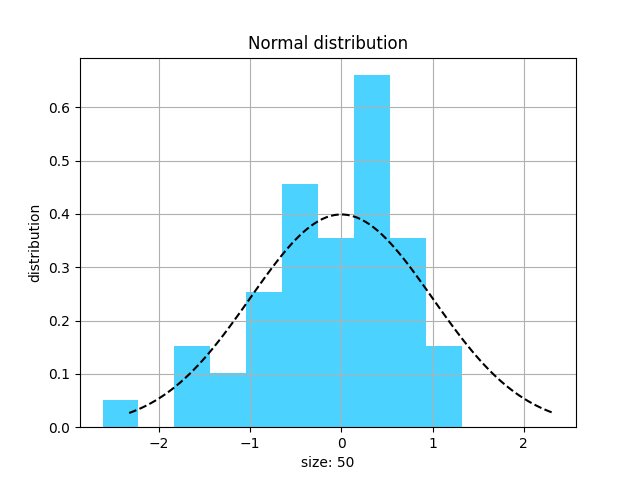
\includegraphics[height = 0.25\textheight, width = 0.31\textwidth]{../image/lab1/lab1_norm_50.png}
			& 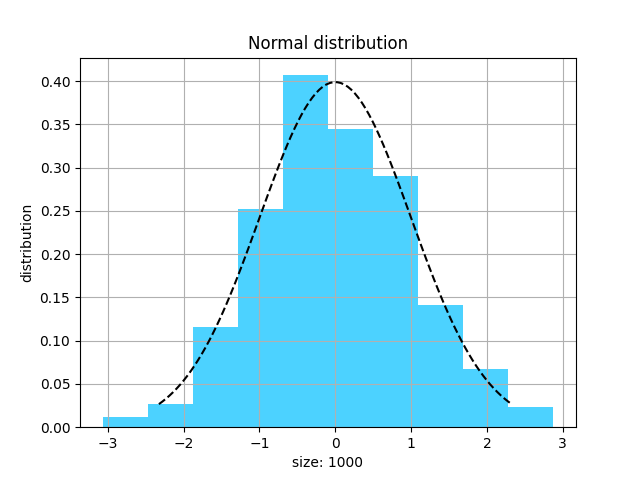
\includegraphics[height = 0.25\textheight, width = 0.31\textwidth]{../image/lab1/lab1_norm_1000.png}
		\end{tabular}
		\caption{Нормальное распределение}
	\end{figure}
	
	\begin{figure}[H]
		\centering
		\begin{tabular}{c c c}
			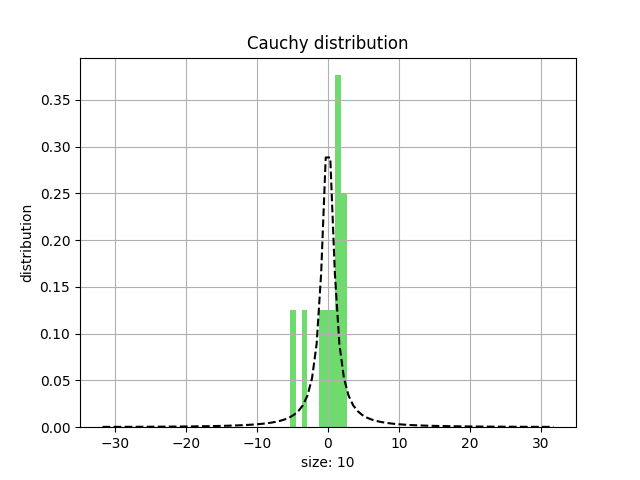
\includegraphics[height = 0.25\textheight, width = 0.31\textwidth]{../image/lab1/lab1_cauchy_10.png}
			& 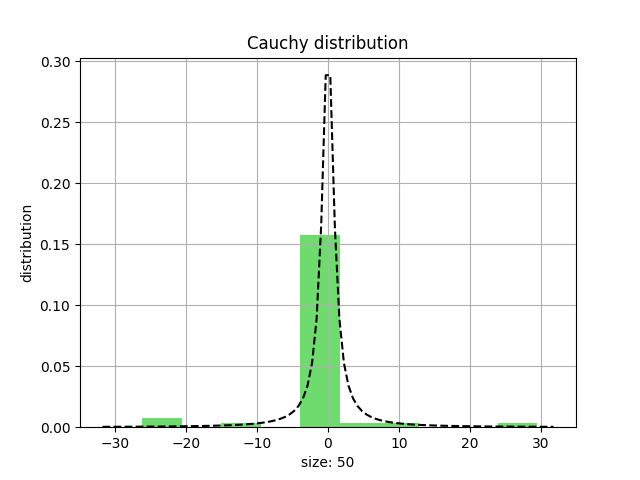
\includegraphics[height = 0.25\textheight, width = 0.31\textwidth]{../image/lab1/lab1_cauchy_50.png}
			& 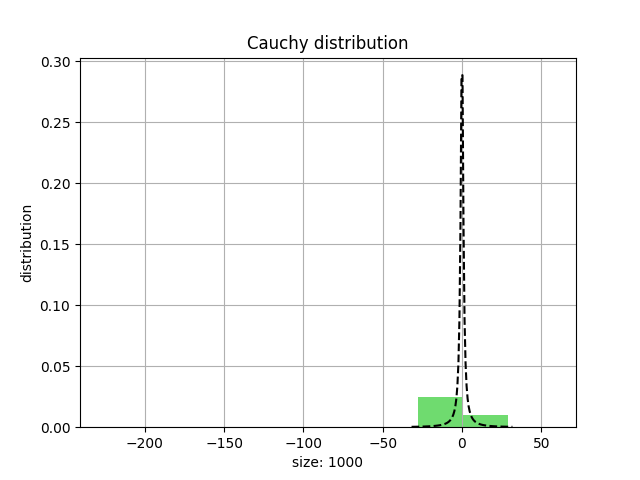
\includegraphics[height = 0.25\textheight, width = 0.31\textwidth]{../image/lab1/lab1_cauchy_1000.png}
		\end{tabular}
		\caption{Распределение Коши}
	\end{figure}
	
	\begin{figure}[H]
		\centering
		\begin{tabular}{c c c}
			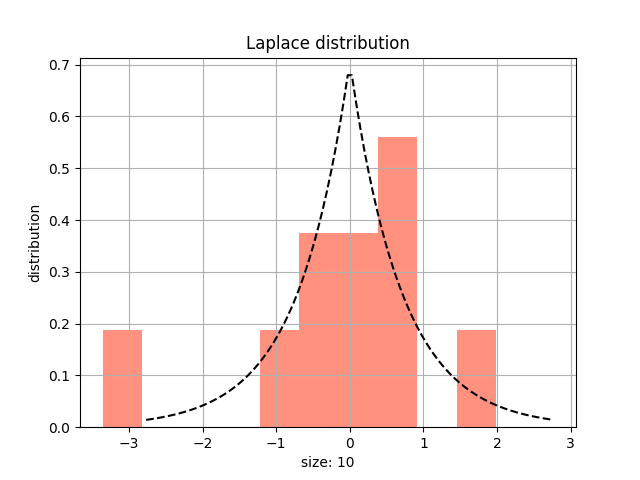
\includegraphics[height = 0.25\textheight, width = 0.31\textwidth]{../image/lab1/lab1_laplace_10.png}
			& 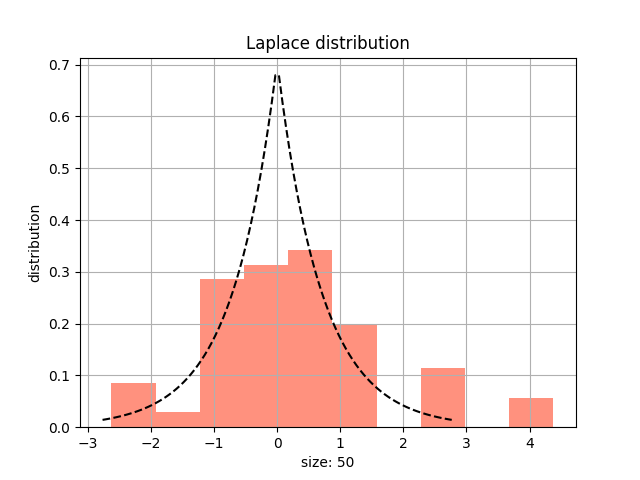
\includegraphics[height = 0.25\textheight, width = 0.31\textwidth]{../image/lab1/lab1_laplace_50.png}
			& 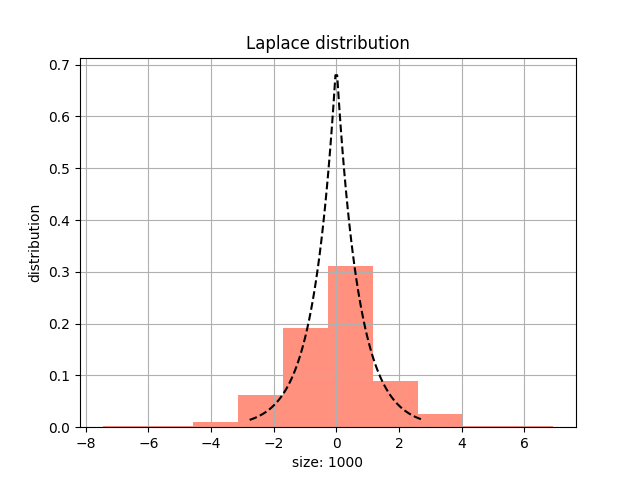
\includegraphics[height = 0.25\textheight, width = 0.31\textwidth]{../image/lab1/lab1_laplace_1000.png}
		\end{tabular}
		\caption{Распределение Лапласа}
	\end{figure}
	
	\begin{figure}[H]
		\centering
		\begin{tabular}{c c c}
			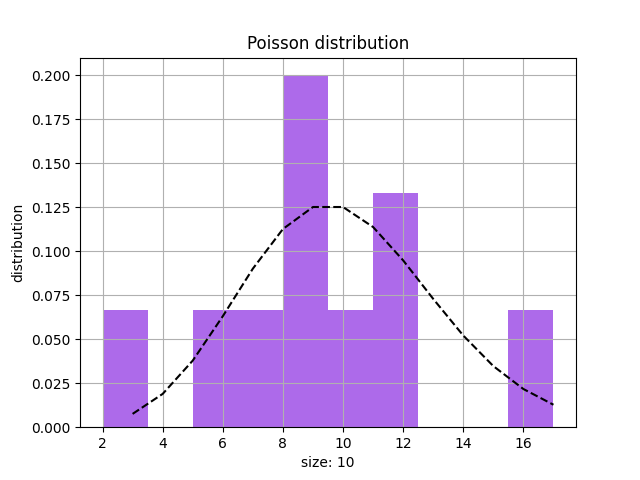
\includegraphics[height = 0.25\textheight, width = 0.31\textwidth]{../image/lab1/lab1_poisson_10.png}
			& 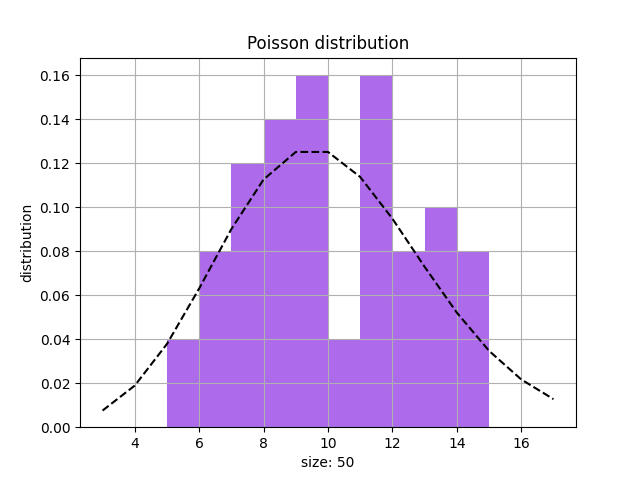
\includegraphics[height = 0.25\textheight, width = 0.31\textwidth]{../image/lab1/lab1_poisson_50.png}
			& 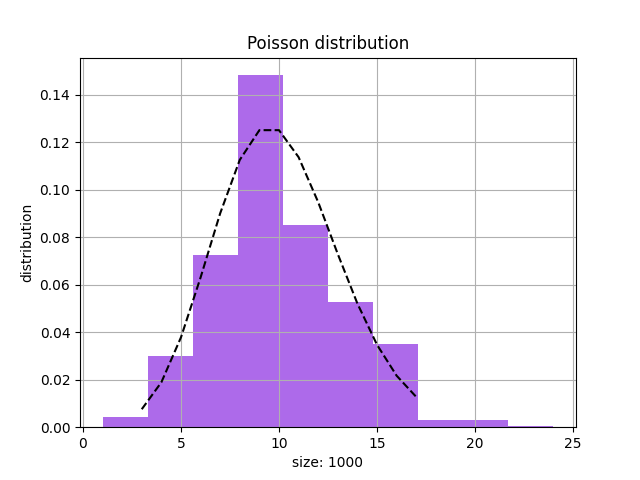
\includegraphics[height = 0.25\textheight, width = 0.31\textwidth]{../image/lab1/lab1_poisson_1000.png}
		\end{tabular}
		\caption{Распределение Пуассона}
	\end{figure}
	
	\begin{figure}[H]
		\centering
		\begin{tabular}{c c c}
			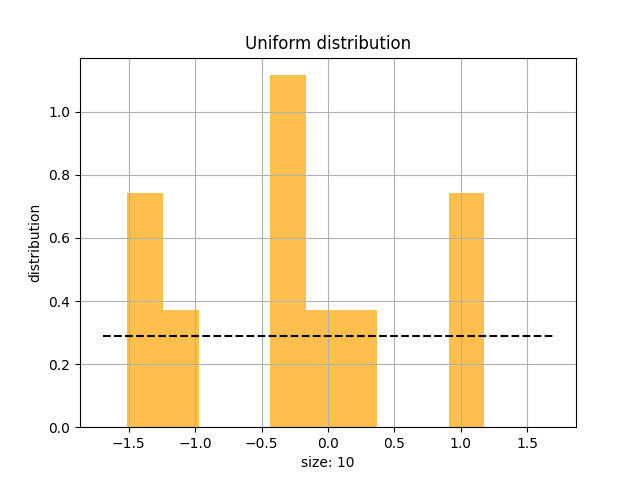
\includegraphics[height = 0.25\textheight, width = 0.31\textwidth]{../image/lab1/lab1_uniform_10.png}
			& 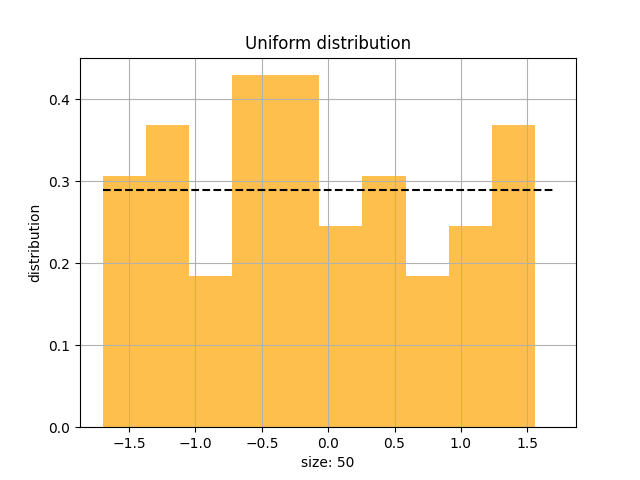
\includegraphics[height = 0.25\textheight, width = 0.31\textwidth]{../image/lab1/lab1_uniform_50.png}
			& 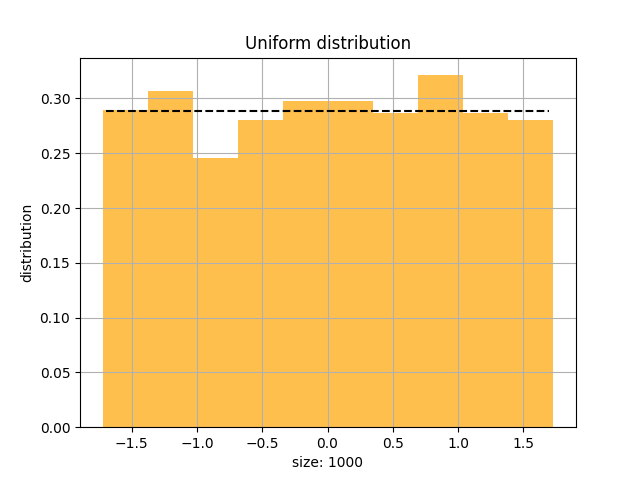
\includegraphics[height = 0.25\textheight, width = 0.31\textwidth]{../image/lab1/lab1_uniform_1000.png}
		\end{tabular}
		\caption{Равномерное распределение}
	\end{figure}
	\subsection{Характеристики положения и рассеяния}
	Как было проведено округление:\\
	В оценке $x=E  \pm D$ вариации подлежит первая цифра после точки. \\
	В данном случае $x=0.0 \pm 0.1k$,\\
	$k$ - зависит от доверительной вероятности и вида распределения (рассматривается в дальнейшем цикле лабораторных работ). \\
	Округление сделано для  $k=1$.
	
	\begin{table}[H]
		\centering
		\begin{tabular}[t]{|l|r|r|r|r|r|}
			\hline
			& $\overline{x}$ & $med x$ & $z_R$ & $z_Q$ & $z_{tr}$\\\hline\hline
			n=10 & & & & &\\\hline
			$E(z)$ & 0.0 & 0.0 & 0.0 & 0.0 & 0.0\\\hline
			$D(z)$ & 0.1 & 0.1 & 0.17 & 0.11 & 0.11\\\hline
			$E(z)\pm\sqrt[]{D(z)}$ & [-0.3; 0.3] & [-0.3; 0.3] & [-0.4; 0.4] & [-0.3; 0.3] & [-0.3; 0.3]\\ \hline
			$\hat{E(z)}$ & 0 & 0 & 0 & 0 & 0\\\hline
			n=100 & & & & &\\\hline
			$E(z)$ & 0.00 & 0.00 & 0.00 & 0.00 & 0.00\\\hline
			$D(z)$ & 0.01 & 0.01 & 0.09 & 0.012 & 0.012\\\hline
			$E(z)\pm\sqrt[]{D(z)}$ & [-0.10; 0.10]& [-0.12; 0.12] & [-0.30; 0.30] & [-0.11; 0.11] & [-0.11; 0.11]\\\hline
			$\hat{E(z)}$ & 0 & 0 & 0 & 0 & 0\\\hline
			n=1000 & & & & &\\\hline
			$E(z)$ & 0.000 & 0.000 & 0.00 & 0.00 & 0.00\\\hline
			$D(z)$ & 0.001 & 0.001 & 0.06 & 0.001 & 0.001\\\hline
			$E(z)\pm\sqrt[]{D(z)}$ & [-0.03; 0.03] & [-0.04; 0.04] & [-0.2; 0.2] & [-0.03; 0.03] & [-0.03; 0.03]\\\hline
			$\hat{E(z)}$ & 0.0 & 0.0 & 0 & 0.0 & 0.0\\\hline
		\end{tabular}
		\caption{Таблица характеристик для нормального распределения}
		\label{tab:normal}
	\end{table}
	
	\begin{table}[H]
		\centering
		\begin{tabular}[t]{|l|r|r|r|r|r|}
			\hline
			& $\overline{x}$ & $med x$ & $z_R$ & $z_Q$ & $z_{tr}$\\\hline\hline
			n=10 & & & & &\\\hline
			$E(z)$ & -0.0738 & -0.0132 & -0.2 & -0.0088 & -0.0109\\\hline
			$D(z)$ & 90.1201 & 0.3801 & 2044.4211 & 1.0132 & 0.557\\\hline
			$E(z)\pm\sqrt[]{D(z)}$ & [-9.567; 9.4193] & [-0.6297; 0.6033] & [-45.4153;  45.0153] & [-1.0153; 0.9978] & [-0.7572; 0.7354] \\\hline
			$\hat{E(z)}$ & -- & 0 & -- & -- & 0\\\hline
			n=100 & & & & &\\\hline
			$E(z)$ & 2.9876 & -0.0003 & 147.3215 & -0.0013 & -0.0009\\\hline
			$D(z)$ & 6138.7132 & 0.0262 & 15314196.8518 & 0.055 & 0.0273\\\hline
			$E(z)\pm\sqrt[]{D(z)}$ & [-75.3623; & [-0.162; & [-3766.0142; & [-0.2358; & [-0.166; \\
			&  81.3376] &  0.1614] & 4060.6573] & 0.2332] & 0.1642]\\\hline
			$\hat{E(z)}$ & -- & 0 & -- & 0 & 0\\\hline
			n=1000 & & & & &\\\hline
			$E(z)$ & 0.1742 & -0.0022 & 105.9198 & -0.0012 & -0.0009\\\hline
			$D(z)$ & 91.5623 & 0.0025 & 21560364.3513 & 0.0049 & 0.0026\\\hline
			$E(z)\pm\sqrt[]{D(z)}$ & [-9.3947; 9.743] & [-0.0522; 0.0478] & [-4537.3941; & [-0.0712; 0.0689] & [-0.0519; 0.0501] \\
			&  &  & 4749.2337] & &\\\hline
			$\hat{E(z)}$ & -- & 0.0 & -- & 0.0 & 0.0\\\hline
		\end{tabular}
		\caption{Таблица характеристик для распределения Коши}
		\label{tab:cauchy}
	\end{table}
	
	\begin{table}[H]
		\centering
		\begin{tabular}[t]{|l|r|r|r|r|r|}
			\hline
			& $\overline{x}$ & $med x$ & $z_R$ & $z_Q$ & $z_{tr}$\\\hline\hline
			n=10 & & & & &\\\hline
			$E(z)$ & 0.00 & 0.00 & 0.00 & 0.00 & 0.00\\\hline
			$D(z)$ & 0.1 & 0.07 & 0.4 & 0.08 & 0.07\\\hline
			$E(z)\pm\sqrt[]{D(z)}$ & [-0.3; 0.3] & [-0.2; 0.2] & [-0.6; 0.6] & [-0.3; 0.3] & [-0.2; 0.2] \\\hline
			$\hat{E(z)}$ & 0 & 0 & 0 & 0 & 0\\\hline
			n=100 & & & & &\\\hline
			$E(z)$ & 0.00 & 0.00 & 0.0 & 0.00 &  0.00\\\hline
			$D(z)$ & 0.01 & 0.006 & 0.4 & 0.01 & 0.006\\\hline
			$E(z)\pm\sqrt[]{D(z)}$ & [-0.1; 0.1] & [-0.07; 0.07] & [-0.6; 0.6] & [-0.1; 0.1] & [-0.08; 0.08]\\\hline
			$\hat{E(z)}$ & 0 & 0.0 & 0 & 0 &  0.0\\\hline
			n=1000 & & & & &\\\hline
			$E(z)$ & 0.00 & 0.00 & 0.0 & 0.00 & 0.00\\\hline
			$D(z)$ & 0.001 & 0.0005 & 0.4 & 0.001 & 0.0006\\\hline
			$E(z)\pm\sqrt[]{D(z)}$ & [-0.03; 0.03]& [-0.02; 0.02] & [-0.6; 0.6] & [-0.03; 0.03] & [-0.02; 0.02] \\\hline
			$\hat{E(z)}$ & 0.0 & 0.0 & 0 & 0.0 &  0.0\\\hline
		\end{tabular}
		\caption{Таблица характеристик для распределения Лапласа}
		\label{tab:laplace}
	\end{table}
	
	\begin{table}[H]
		\centering
		\begin{tabular}[t]{|l|r|r|r|r|r|}
			\hline
			& $\overline{x}$ & $med x$ & $z_R$ & $z_Q$ & $z_{tr}$\\\hline\hline
			n=10 & & & & &\\\hline
			$E(z)$ & 10.0 & 9.8 & 10.3 & 9.9 & 9.9\\\hline
			$D(z)$ & 1.0 & 1.4 & 1.8 & 1.1 & 1.1\\\hline
			$E(z)\pm\sqrt[]{D(z)}$ & [9.0; 11.0] & [8.6; 11.0] & [8.9; 11.7] & [8.8; 11.0] & [8.8; 10.9] \\\hline
			$\hat{E(z)}$ & -- & -- & -- & -- &  --\\\hline
			n=100 & & & & &\\\hline
			$E(z)$ & 10.0 & 9.8 & 10.9 & 9.9 & 9.8\\\hline
			$D(z)$ & 0.1 & 0.2 & 1.0 & 0.15 & 0.1\\\hline
			$E(z)\pm\sqrt[]{D(z)}$ & [9.6; 10.3] & [9.4; 10.3] & [9.9; 11.9] & [9.5; 10.3] & [9.5; 10.2]\\\hline
			$\hat{E(z)}$ & -- & -- & -- & -- &  --\\\hline
			n=1000 & & & & &\\\hline
			$E(z)$ & 10.00 & 9.99 & 11.6 & 9.99 & 9.85\\\hline
			$D(z)$ & 0.010 & 0.0002 & 0.6 & 0.002 & 0.011\\\hline
			$E(z)\pm\sqrt[]{D(z)}$ & [9.90; 10.09] & [9.9; 10.0] & [10.8; 12.4] & [9.94; 10.04] & [9.75; 9.96] \\\hline
			$\hat{E(z)}$ & -- & -- & -- & -- &  9 \\\hline
		\end{tabular}
		\caption{Таблица характеристик для распределения Пуассона}
		\label{tab:poisson}
	\end{table}
	
	\begin{table}[H]
		\centering
		\begin{tabular}[t]{|l|r|r|r|r|r|}
			\hline
			& $\overline{x}$ & $med x$ & $z_R$ & $z_Q$ & $z_{tr}$\\\hline\hline
			n=10 & & & & &\\\hline
			$E(z)$ & 0.00 & 0.00 & 0.00 & 0.00 & 0.00\\\hline
			$D(z)$ & 0.09 & 0.22 & 0.04 & 0.13 & 0.16\\\hline
			$E(z)\pm\sqrt[]{D(z)}$ & [-0.31; 0.31] & [-0.47; 0.47] & [-0.20; 0.20] & [-0.37; 0.37] & [-0.40; 0.40]\\\hline
			$\hat{E(z)}$ & 0 & 0 & 0 & 0 &  0\\\hline
			n=100 & & & & &\\\hline
			$E(z)$ & 0.00 & 0.00 & 0.00 & 0.00 & 0.00\\\hline
			$D(z)$ & 0.010 & 0.028 & 0.0006 & 0.014 & 0.019\\\hline
			$E(z)\pm\sqrt[]{D(z)}$ & [-0.10; 0.10] & [-0.16; 0.16] & [-0.02; 0.02] & [-0.12; 0.12] & [-0.13; 0.13] \\\hline
			$\hat{E(z)}$ & 0 & 0 & 0.0 & 0 &  0\\\hline
			n=1000 & & & & &\\\hline
			$E(z)$ & 0.00 & 0.00 & 0.000 & 0.00 & 0.00\\\hline
			$D(z)$ & 0.001 & 0.003 & 0.000 & 0.0015 & 0.002\\\hline
			$E(z)\pm\sqrt[]{D(z)}$ & [-0.03; 0.03] & [-0.05; 0.05] & [-0.0025; 0.0025] & [-0.03; 0.03] & [-0.04; 0.04] \\\hline
			$\hat{E(z)}$ & 0.0 & 0.0 & 0.00 & 0.0 &  0.0\\\hline
		\end{tabular}
		\caption{Таблица характеристик для равномерного распределения}
		\label{tab:uniform}
	\end{table}
	\subsection{Боксплот Тьюки}
	\begin{figure}[H]
		\centering
		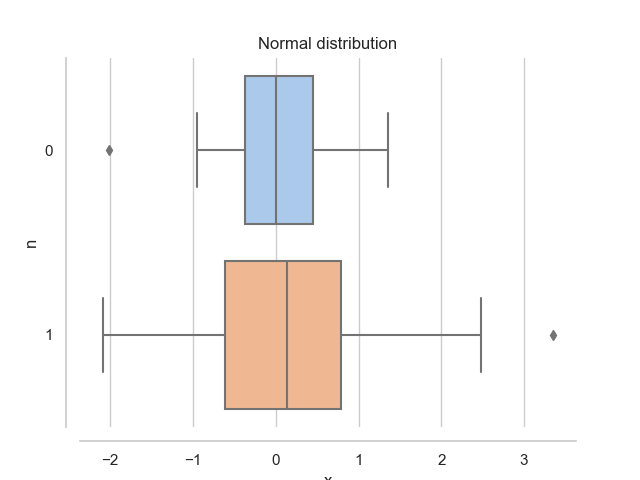
\includegraphics[scale=0.6]{../image/lab3/lab3_norm.png}
		\caption{Нормальное распределение}
		\label{fig:normal}
	\end{figure}
	
	\begin{figure}[H]
		\centering
		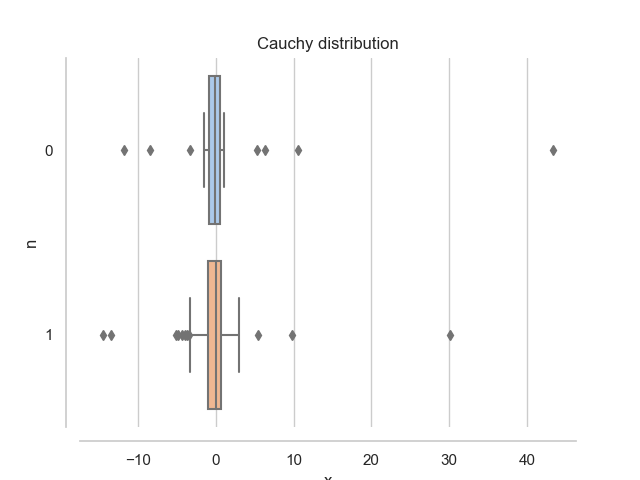
\includegraphics[scale=0.6]{../image/lab3/lab3_cauchy.png}
		\caption{Распределение Коши}
		\label{fig:cauchy}
	\end{figure}
	
	\begin{figure}[H]
		\centering
		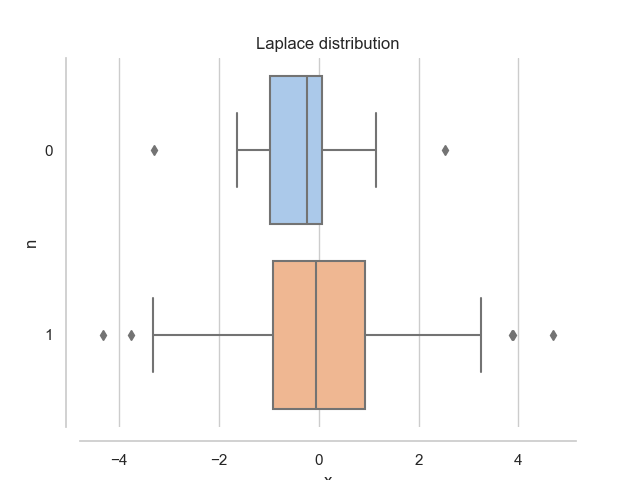
\includegraphics[scale=0.6]{../image/lab3/lab3_laplace.png}
		\caption{Распределение Лапласа}
		\label{fig:laplace}
	\end{figure}
	
	\begin{figure}[H]
		\centering
		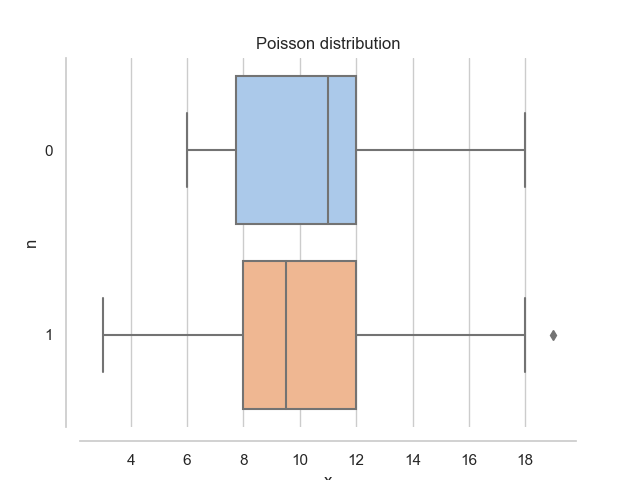
\includegraphics[scale=0.6]{../image/lab3/lab3_poisson.png}
		\caption{Распределение Пуассона}
		\label{fig:poisson}
	\end{figure}
	
	\begin{figure}[H]
		\centering
		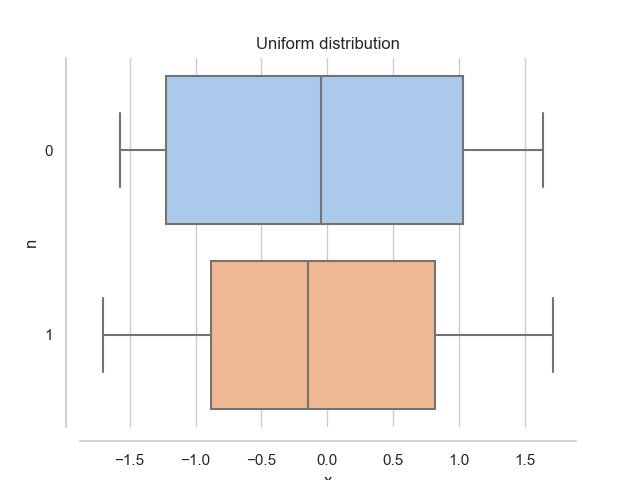
\includegraphics[scale=0.6]{../image/lab3/lab3_uniform.png}
		\caption{Равномерное распределение}
		\label{fig:uniform}
	\end{figure}
	\subsection{Доля выбросов}
	Выборка случайна, поэтому в качестве оценки рассеяния можно взять дисперсию пуассоновского потока:  $D_n \approx \sqrt{n}$\\
	Доля $p_n = \frac{D_n}{n}=\frac{1}{\sqrt{n}}$\\
	Доля $n=20: p_n=\frac{1}{\sqrt{20}}$ - примерно 0.2 или 20\% \\
	Для $n=100: p_n=\frac{1}{\sqrt{100}}$ - примерно 0.1 или 10\% \\
	Исходя из этого можно решить, сколько знаков оставлять в доле выброса.
	
	\begin{table}[H]
		\centering
		\begin{tabular}{|l|c|c|}
			\hline
			Выборка & Доля выбросов	& $P^T_B$\\\hline
			\hline
			Normal n = 20 & 0.0257 & 0.007\\\hline
			Normal n = 100 & 0.01083 & 0.007\\\hline
			Cauchy n = 20 & 0.1514 & 0.156\\\hline
			Cauchy n = 100 & 0.15418 & 0.156\\\hline
			Laplace n = 20 & 0.0701 & 0.063\\\hline
			Laplace n = 100 & 0.06534 & 0.063\\\hline
			Poisson n = 20 & 0.0247 & 0.008\\\hline
			Poisson n = 100 & 0.0106 & 0.008\\\hline
			Uniform n = 20 & 0.00225 & 0\\\hline
			Uniform n = 100 & 0 & 0\\\hline
		\end{tabular}
		\caption{Практическая доля выбросов}
	\end{table}
	\subsection{Теоретическая вероятность выбросов}
	\begin{table}[H]
		\centering
		\begin{tabular}{|l|c|c|c|c|c|}
			\hline
			Распределение & $Q_1^T$	& $Q_3^T$ & $X_1^T$ & $X_2^T$ & $P_B^T$\\\hline
			\hline
			Нормальное & -0.674 & 0.674 & -2.698 &  2.698 & 0.007\\\hline
			Коши & -1 & 1 & -4 & 4 & 0.156\\\hline
			Лапласа & -0.490 & 0.490 & -1.961 & 1.961 & 0.063\\\hline
			Пуассона & 8 & 12 & 2 & 18 & 0.008\\\hline
			Равномерное & -0.866 & 0.866 & -3.464 & 3.464 & 0\\\hline
		\end{tabular}
		\caption{Теоретическая вероятность выбросов}
	\end{table}
	
	\subsection{Эмпирическая функция распределения}
	\begin{figure}[H]
		\centering
		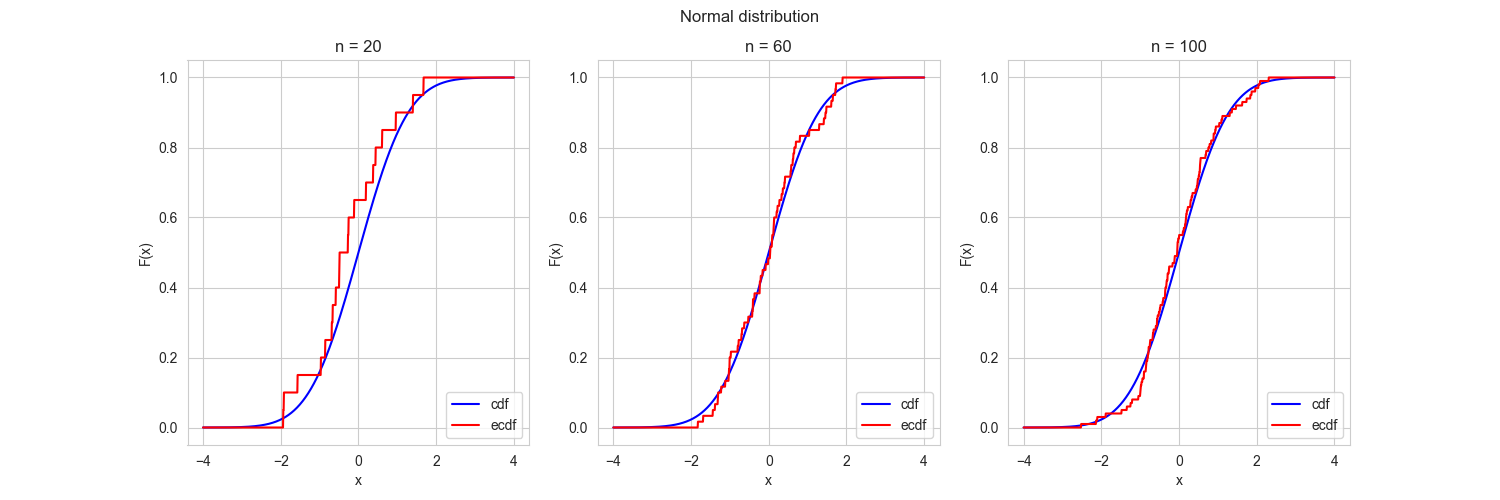
\includegraphics[scale=0.35]{../image/lab4/lab4_ecdf_norm.png}
		\caption{Нормальное распределение}
	\end{figure}
	
	\begin{figure}[H]
		\centering
		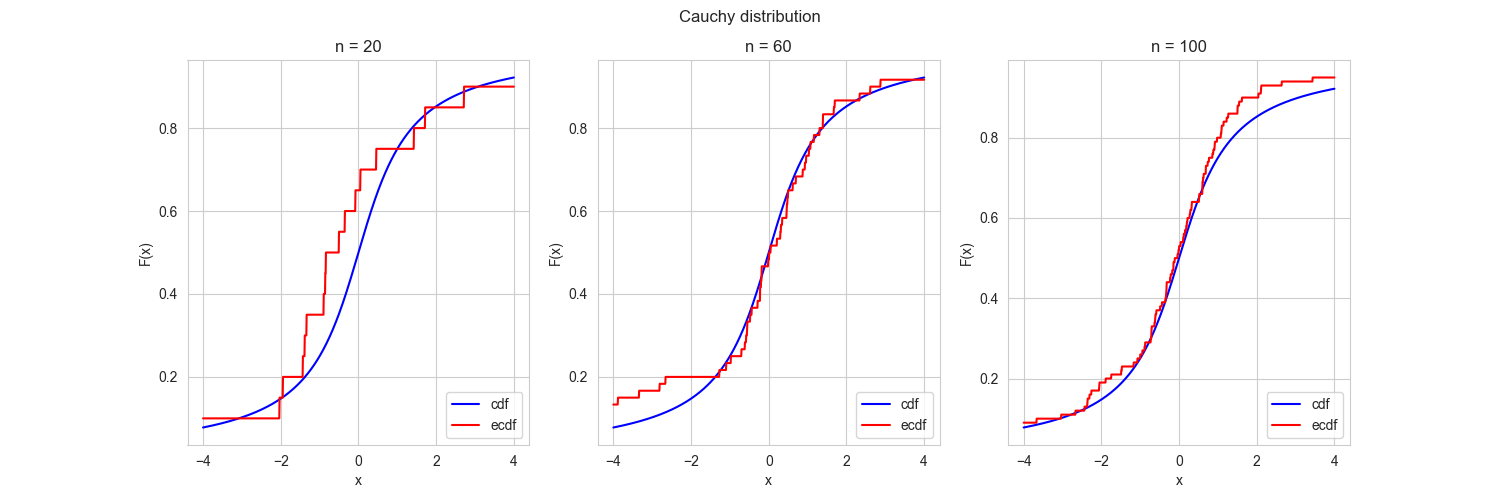
\includegraphics[scale=0.35]{../image/lab4/lab4_ecdf_cauchy.png}
		\caption{Распределение Коши}
	\end{figure}
	
	\begin{figure}[H]
		\centering
		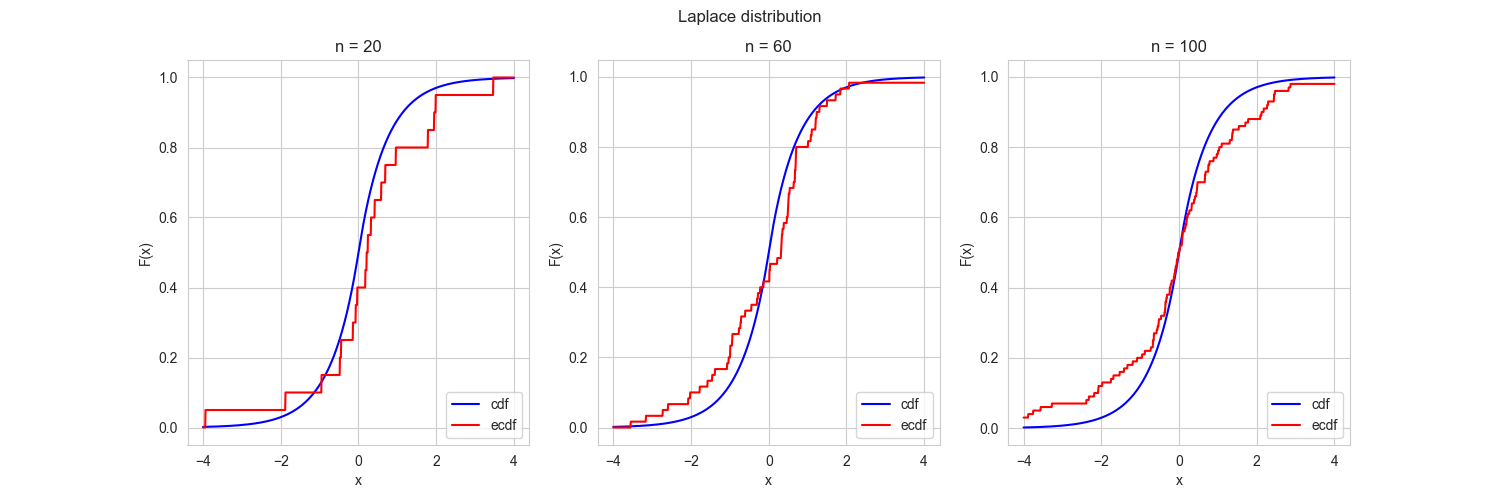
\includegraphics[scale=0.35]{../image/lab4/lab4_ecdf_laplace.png}
		\caption{Распределение Лапласа}
	\end{figure}
	
	\begin{figure}[H]
		\centering
		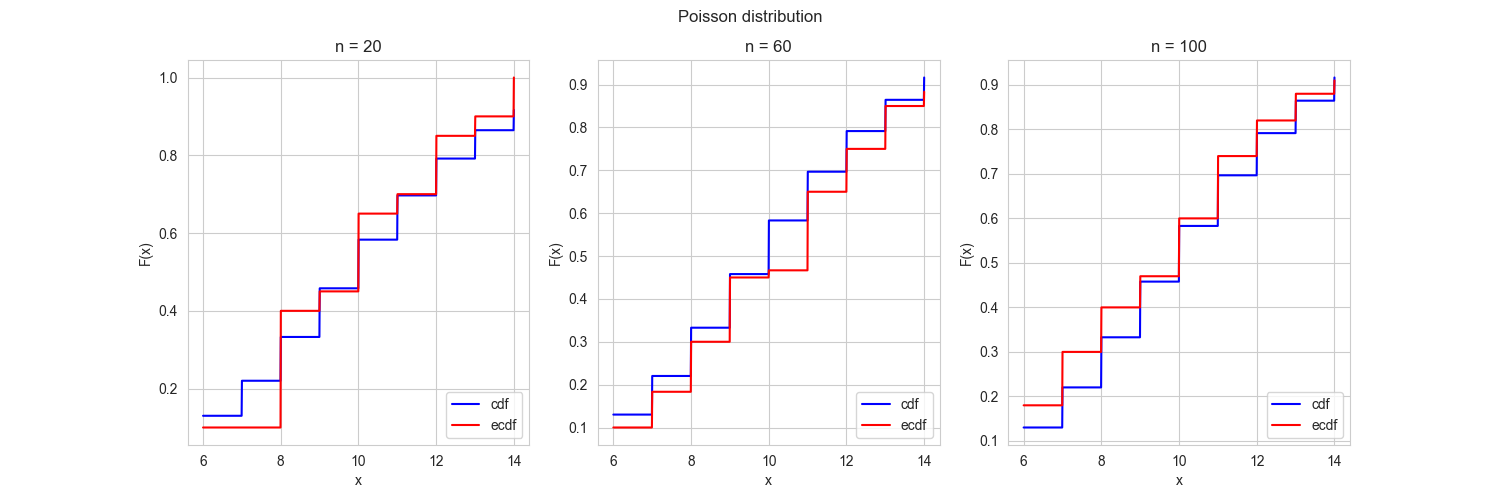
\includegraphics[scale=0.35]{../image/lab4/lab4_ecdf_poisson.png}
		\caption{Распределение Пуассона}
	\end{figure}
	
	\begin{figure}[H]
		\centering
		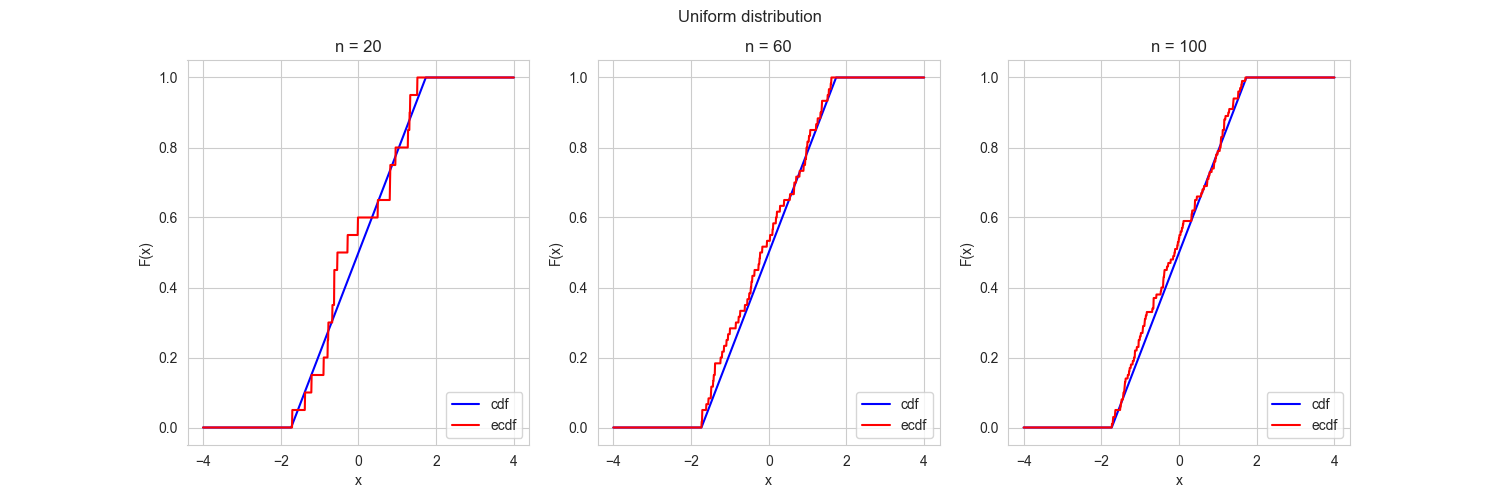
\includegraphics[scale=0.35]{../image/lab4/lab4_ecdf_uniform.png}
		\caption{Равномерное распределение}
	\end{figure}
	\subsection{Ядерные оценки плотности распределения}
	\begin{figure}[H]
		\centering
		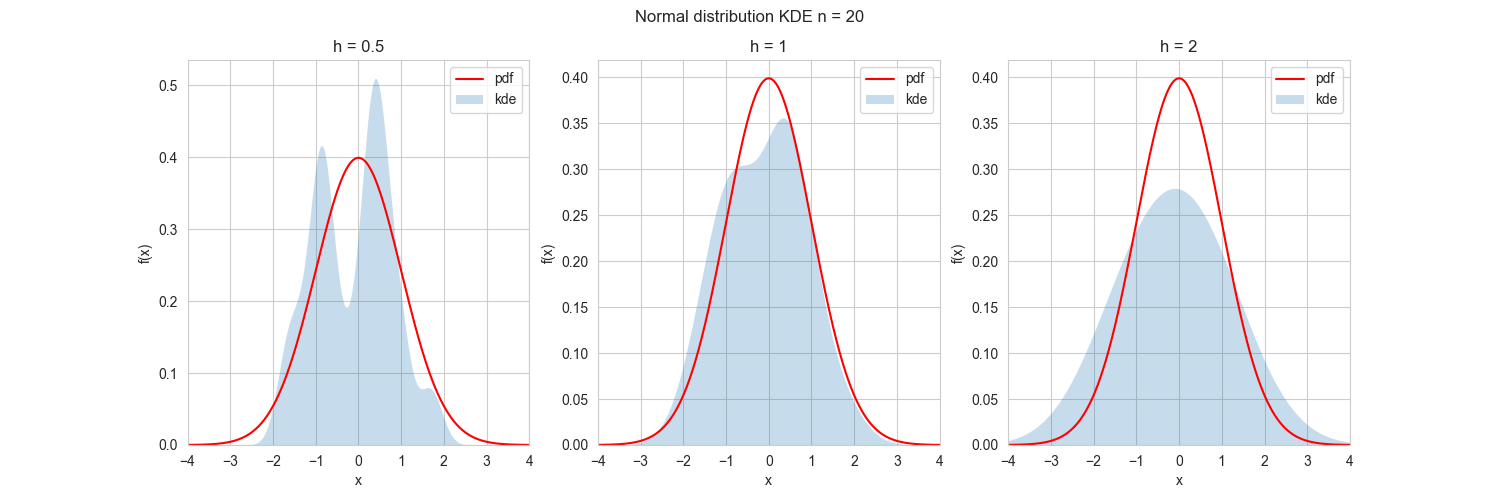
\includegraphics[scale=0.35]{../image/lab4/lab4_kde_norm_20.png}
		\caption{Нормальное распределение размерностью 20}
	\end{figure}
	
	\begin{figure}[H]
		\centering
		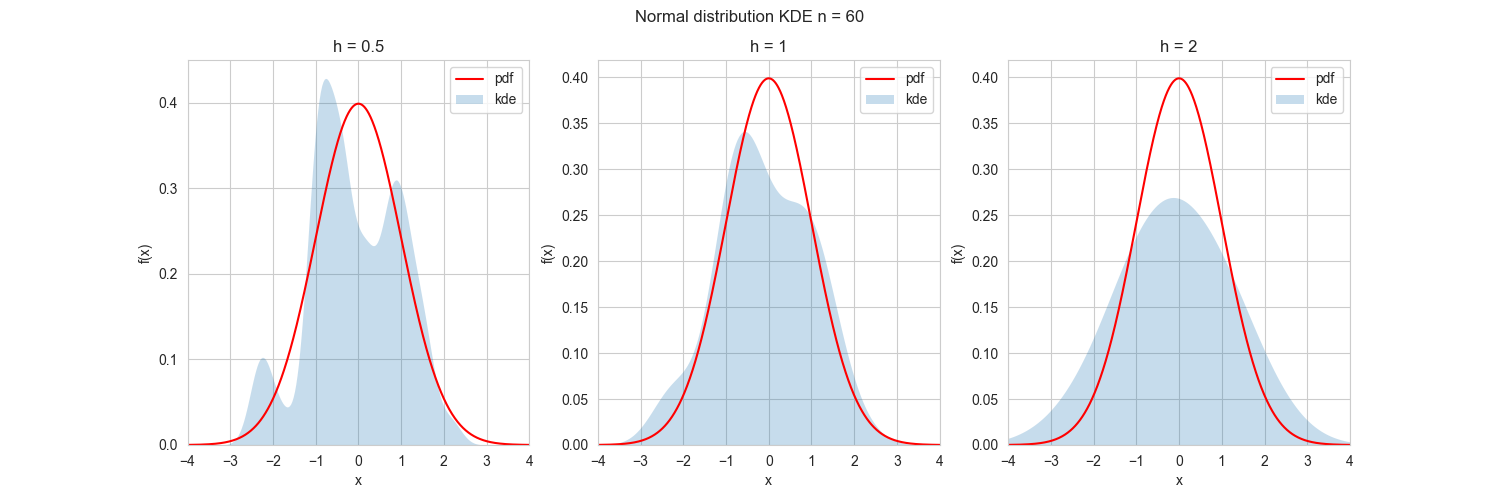
\includegraphics[scale=0.35]{../image/lab4/lab4_kde_norm_60.png}
		\caption{Нормальное распределение размерностью 60}
	\end{figure}
	
	\begin{figure}[H]
		\centering
		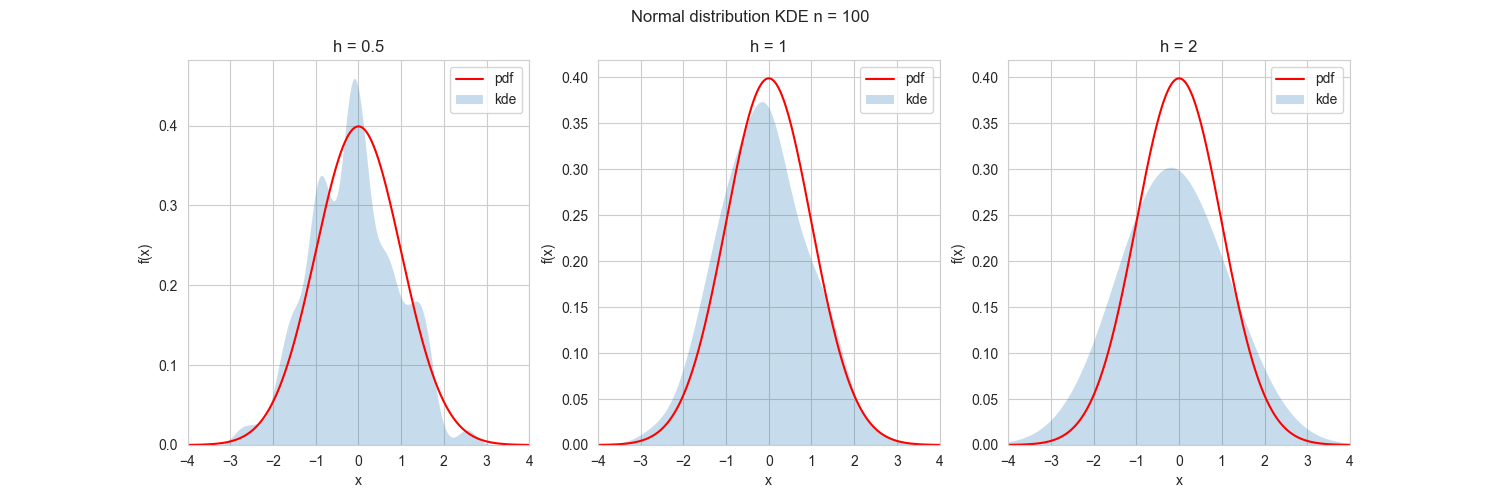
\includegraphics[scale=0.35]{../image/lab4/lab4_kde_norm_100.png}
		\caption{Нормальное распределение размерностью 100}
	\end{figure}
	
	\begin{figure}[H]
		\centering
		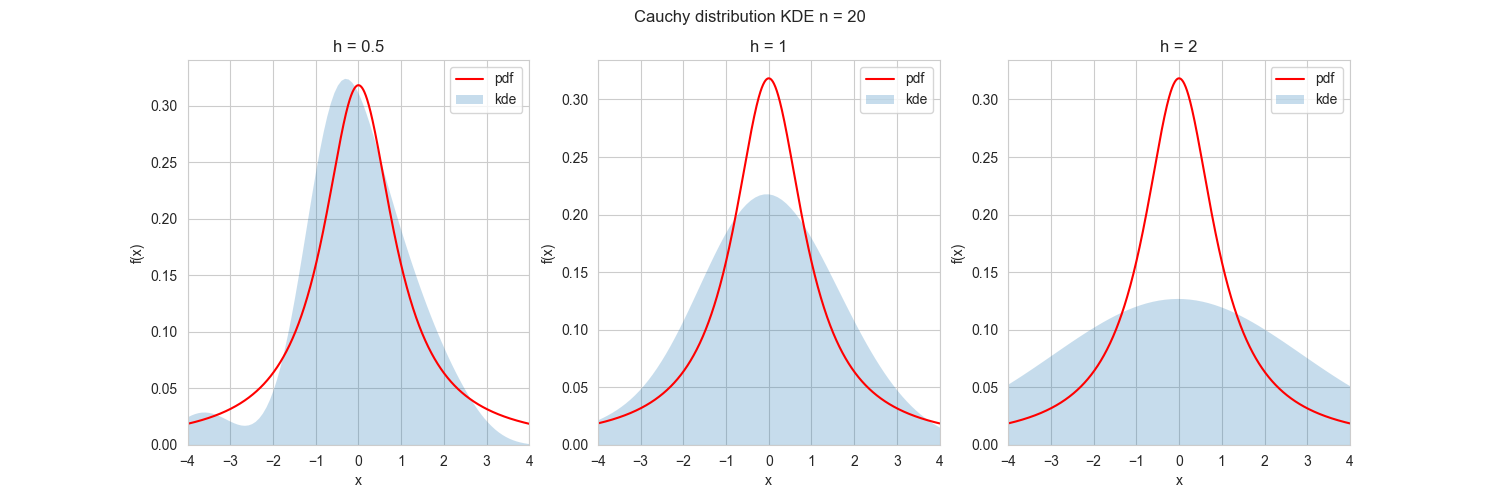
\includegraphics[scale=0.35]{../image/lab4/lab4_kde_cauchy_20.png}
		\caption{Распределение Коши размерностью 20}
	\end{figure}
	
	\begin{figure}[H]
		\centering
		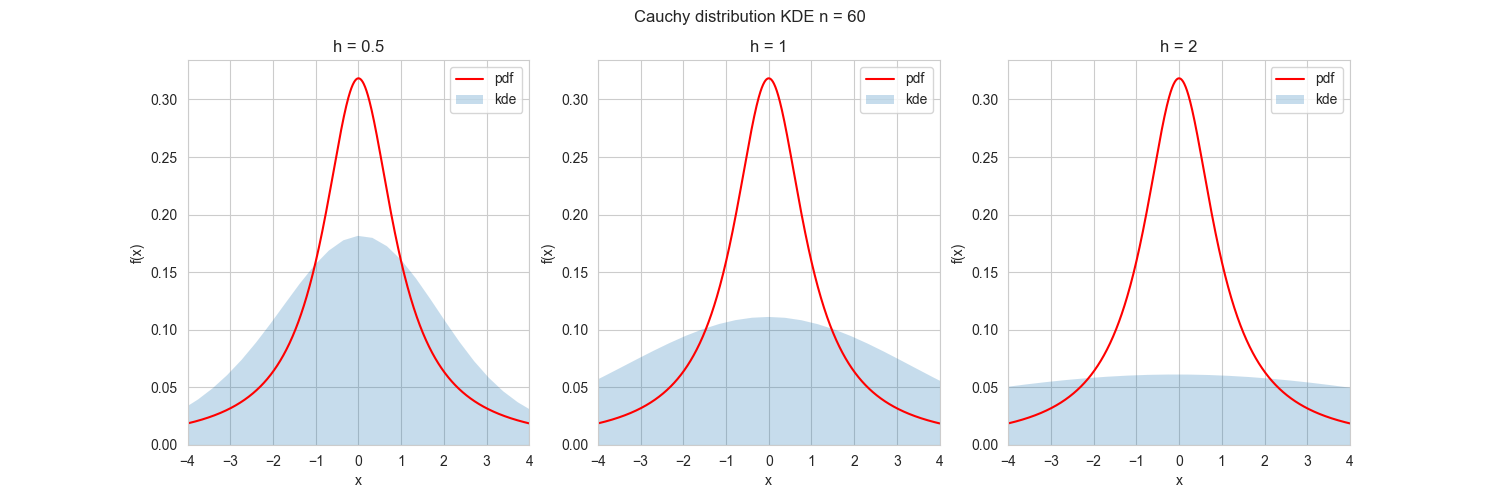
\includegraphics[scale=0.35]{../image/lab4/lab4_kde_cauchy_60.png}
		\caption{Распределение Коши размерностью 60}
	\end{figure}
	
	\begin{figure}[H]
		\centering
		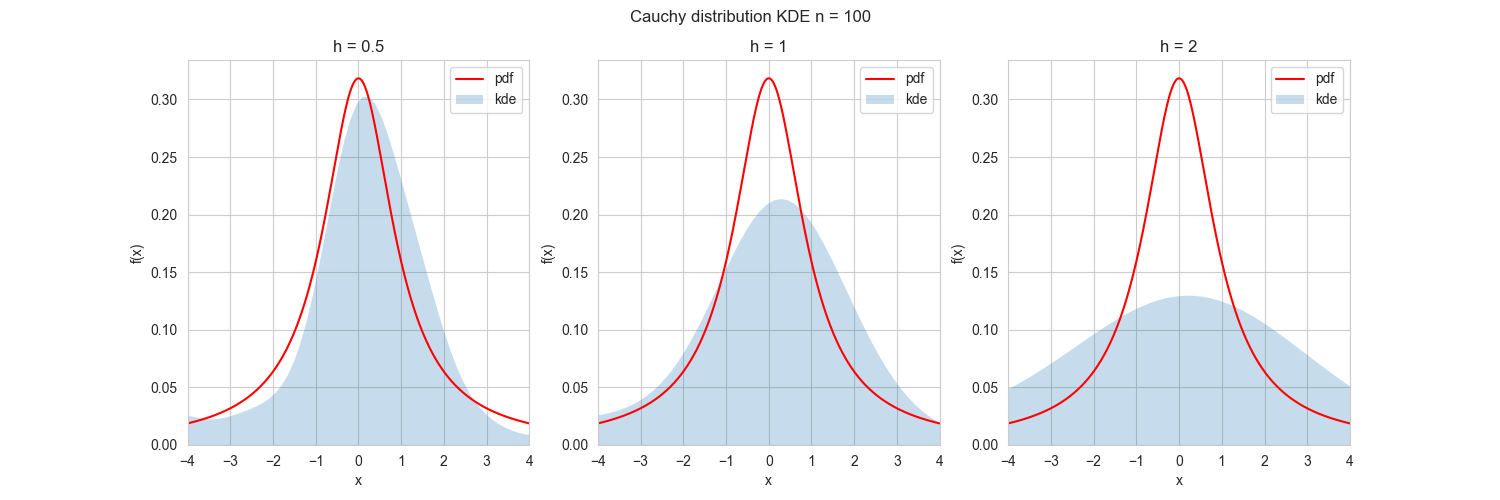
\includegraphics[scale=0.35]{../image/lab4/lab4_kde_cauchy_100.png}
		\caption{Распределение Коши размерностью 100}
	\end{figure}
	
	\begin{figure}[H]
		\centering
		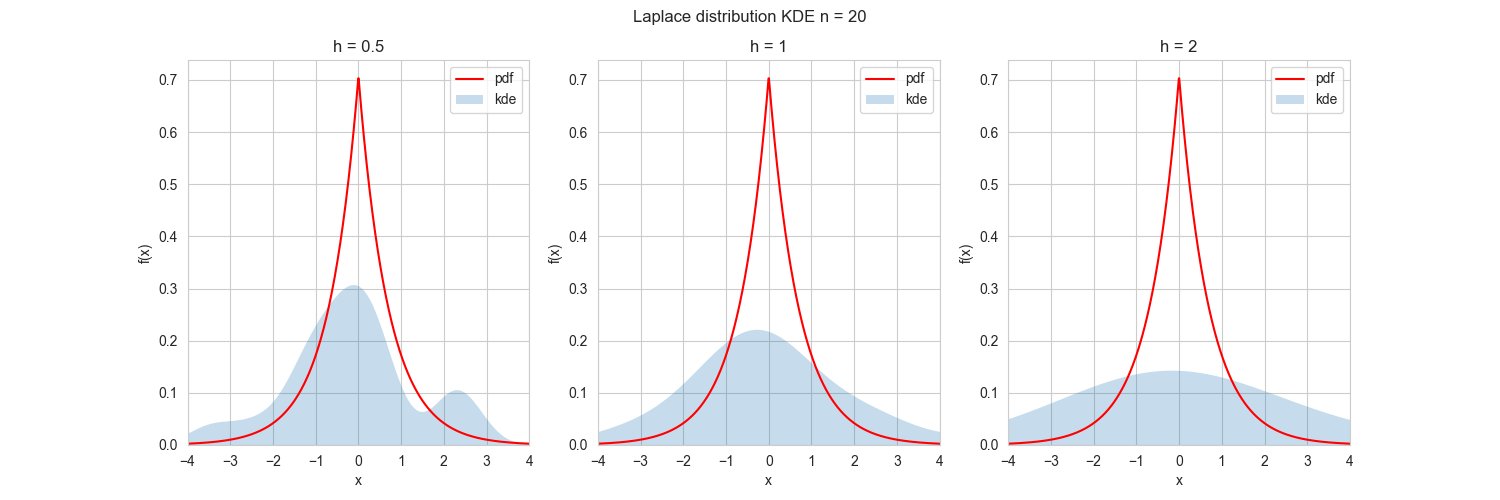
\includegraphics[scale=0.35]{../image/lab4/lab4_kde_laplace_20.png}
		\caption{Распределение Лапласа размерностью 20}
	\end{figure}
	
	\begin{figure}[H]
		\centering
		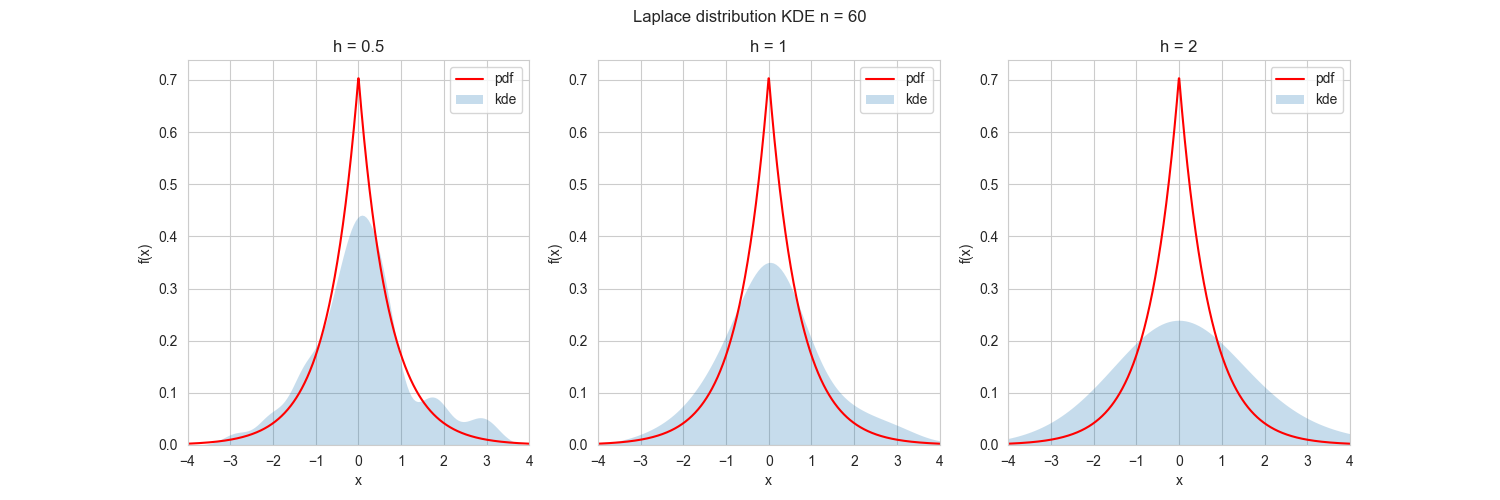
\includegraphics[scale=0.35]{../image/lab4/lab4_kde_laplace_60.png}
		\caption{Распределение Лапласа размерностью 60}
	\end{figure}
	
	\begin{figure}[H]
		\centering
		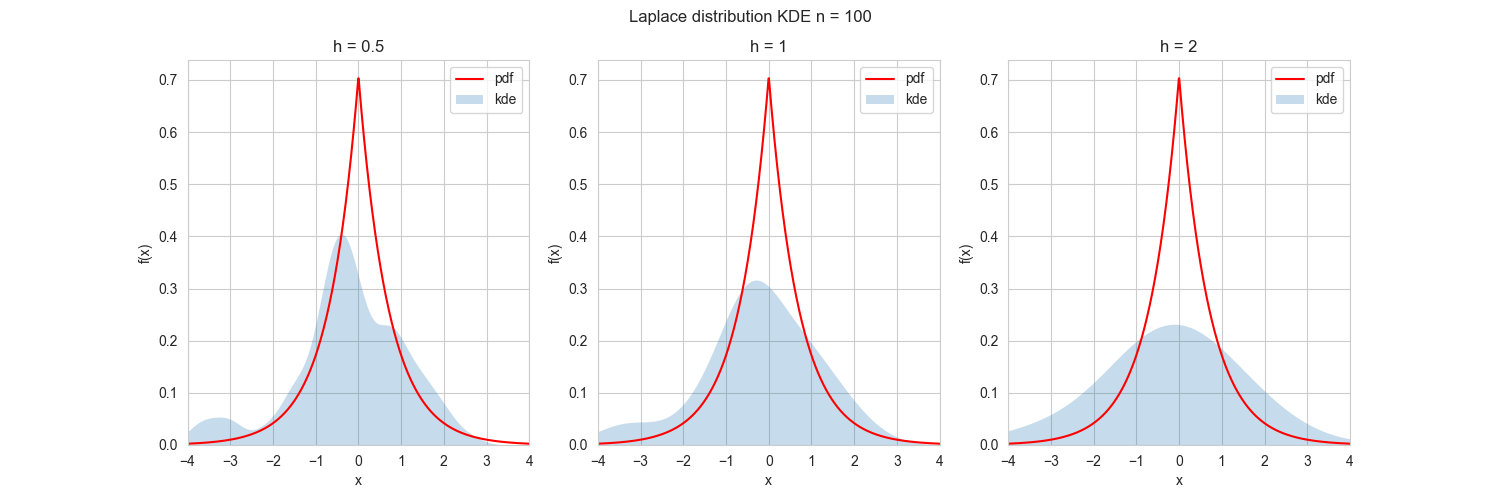
\includegraphics[scale=0.35]{../image/lab4/lab4_kde_laplace_100.png}
		\caption{Распределение Лапласа размерностью 100}
	\end{figure}
	
	\begin{figure}[H]
		\centering
		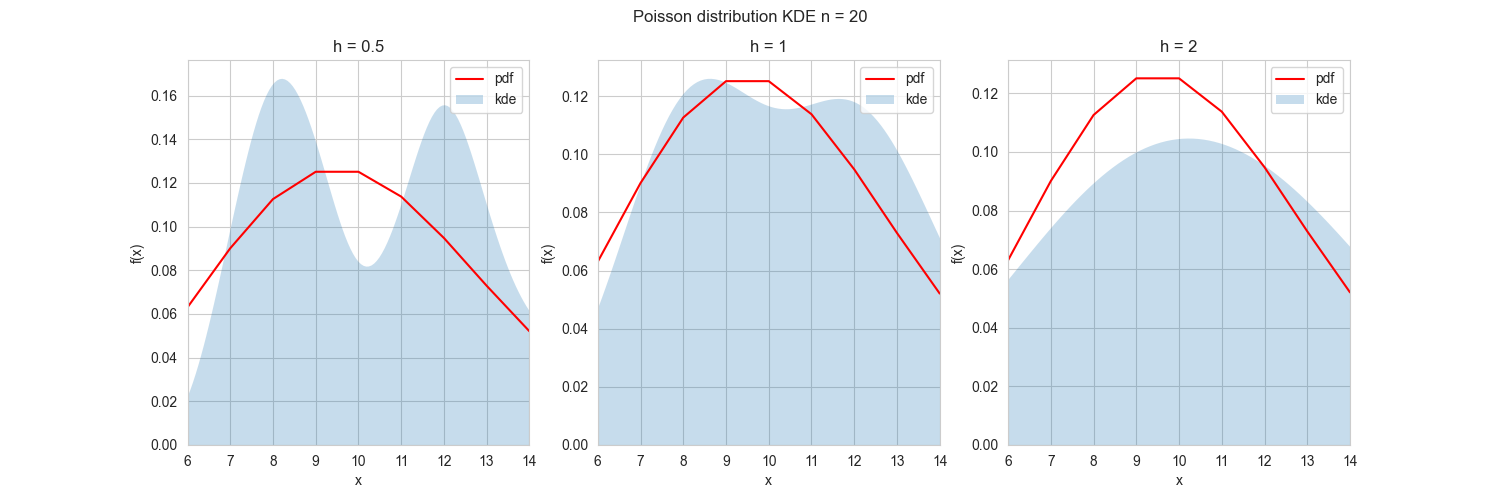
\includegraphics[scale=0.35]{../image/lab4/lab4_kde_poisson_20.png}
		\caption{Распределение Пуассона размерностью 20}
	\end{figure}
	
	\begin{figure}[H]
		\centering
		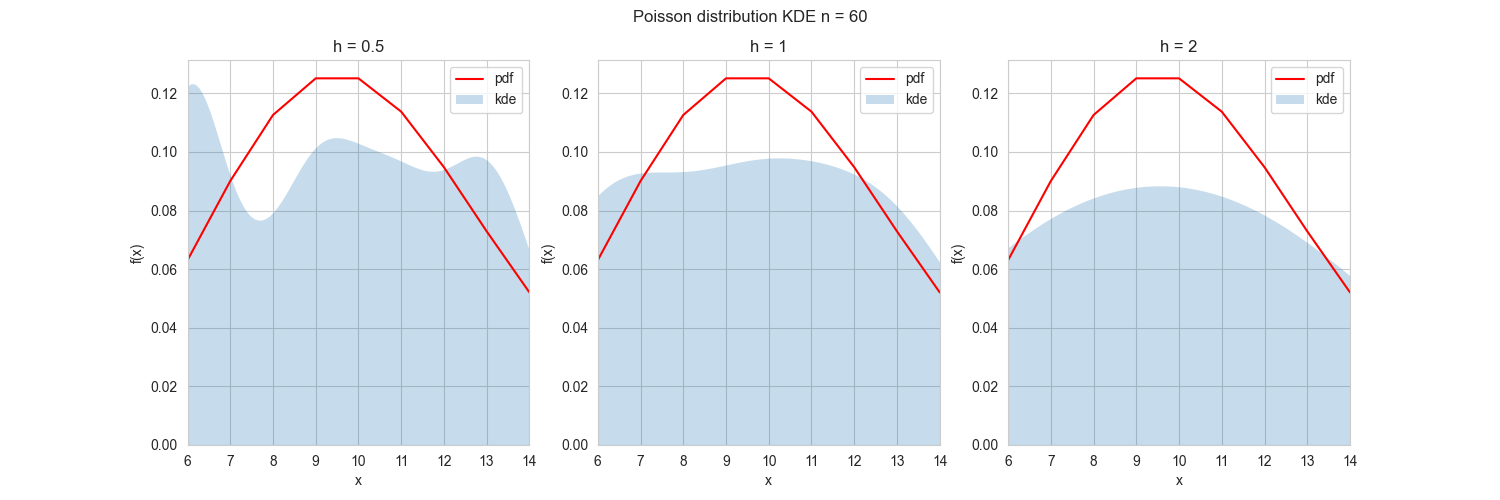
\includegraphics[scale=0.35]{../image/lab4/lab4_kde_poisson_60.png}
		\caption{Распределение Пуассона размерностью 60}
	\end{figure}
	
	\begin{figure}[H]
		\centering
		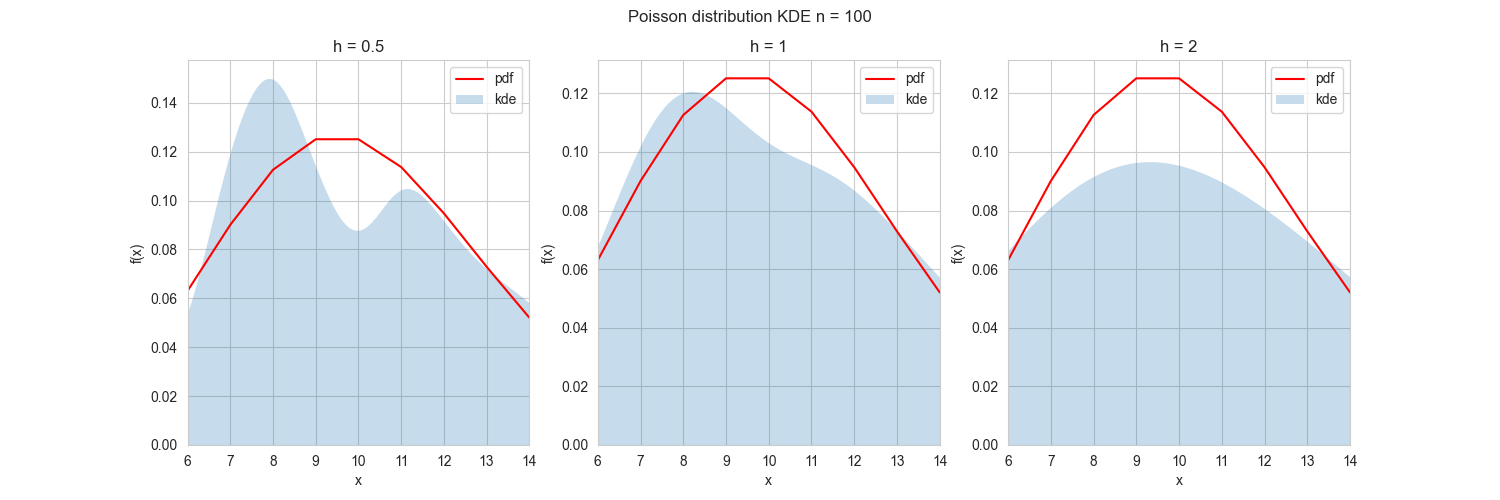
\includegraphics[scale=0.35]{../image/lab4/lab4_kde_poisson_100.png}
		\caption{Распределение Пуассона размерностью 100}
	\end{figure}
	
	\begin{figure}[H]
		\centering
		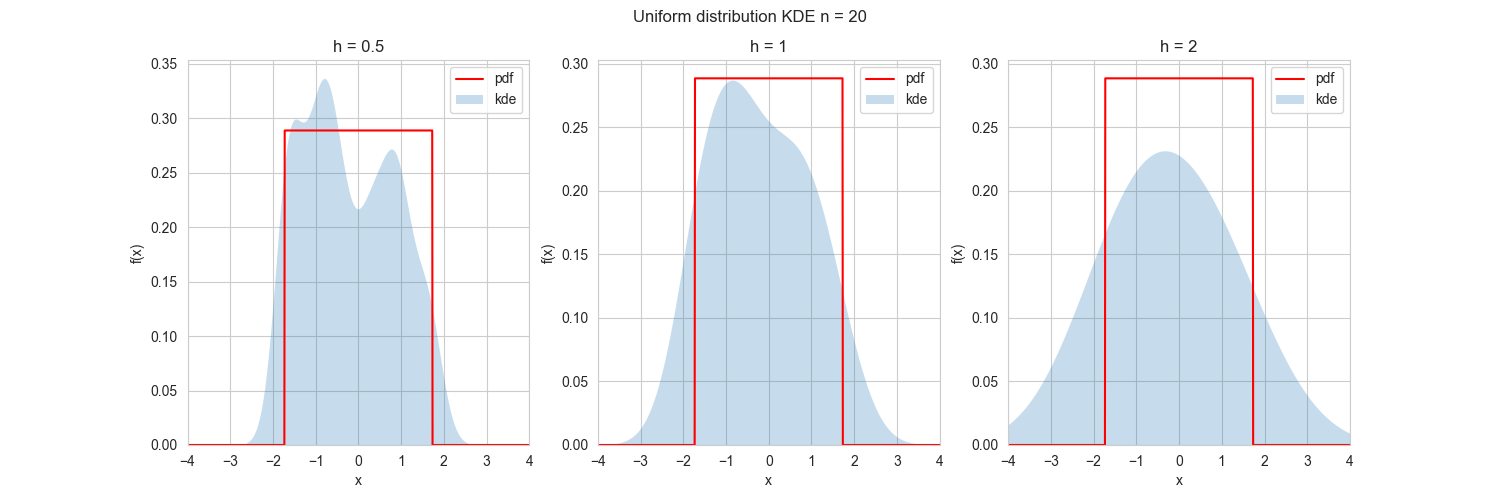
\includegraphics[scale=0.35]{../image/lab4/lab4_kde_uniform_20.png}
		\caption{Равномерное распределение размерностью 20}
	\end{figure}
	
	\begin{figure}[H]
		\centering
		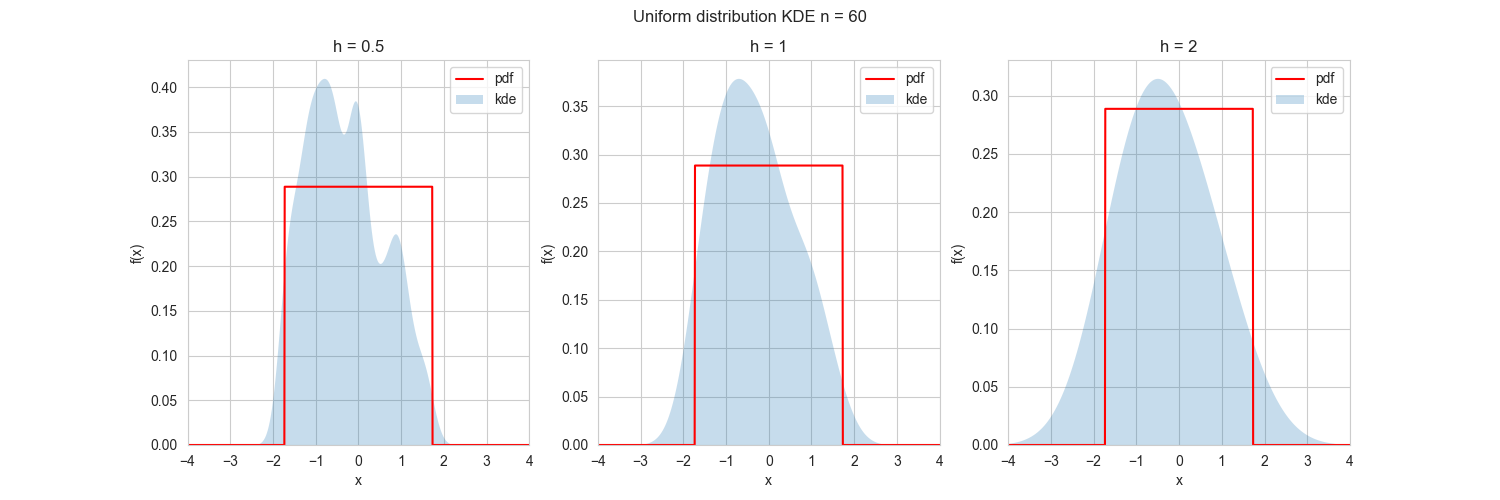
\includegraphics[scale=0.35]{../image/lab4/lab4_kde_uniform_60.png}
		\caption{Равномерное распределение размерностью 60}
	\end{figure}
	
	\begin{figure}[H]
		\centering
		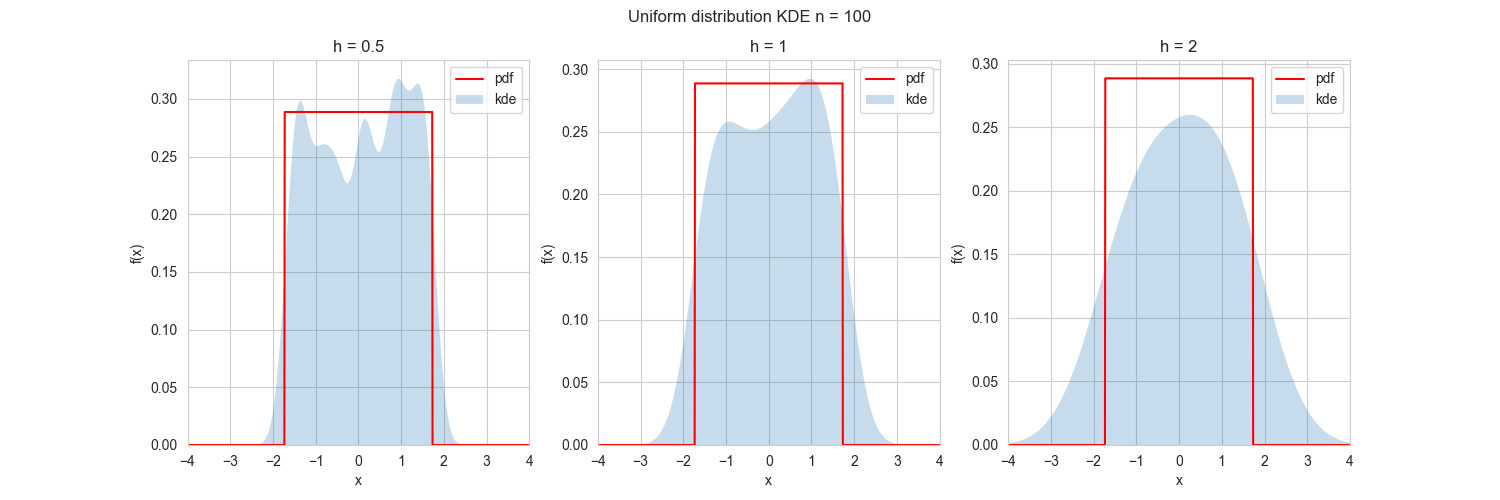
\includegraphics[scale=0.35]{../image/lab4/lab4_kde_uniform_100.png}
		\caption{Равномерное распределение размерностью 100}
	\end{figure}
	
	\section{Обсуждение}
	\subsection{Гистограмма и график плотности распределения}
	Анализ результатов показывает, что чем больше выборка из распределения, тем больше соответсвует гистограмма распределения графику плотности его распределения.\\
	Аналогично можем сказать, что чем больше выборка, тем более заметен характер распределения.
	~\\
	~\\
	Стоит отметить, что распределение Пуассона является более широким, что можно выделить, как отличительную черту распределения. Аналогично для равномерного распределения характерно наличие столбцов более или менее однородной высоты. 
	~\\
	~\\
	На гистограммах наблюдаются всплески, явно превыщающие исходное значение плотности распределения в заданной точке, что наиболее хорошо прослеживается на распределении Коши.
	
	\subsection{Характеристики положения и рассеяния}
	Проанализировав полученные результаты, можно заметить, что для нормального распределения, распределения Лапласа и равномерного распределения $E(z)$ и $D(z)$ для всех характеристик уменьшается с ростом выборки.
	~\\
	~\\
	Стоит отметить, что в распределении Пуассона $E(z)$ для всех характеристик колеблется  в окрестности 10, по $D(z)$, аналогично рассмотренным выше распределениям, наблюдается уменьшение значений при росте выборки.
	~\\
	~\\
	К тому же, в таблице характеристик распределения Коши можно выделить аномальные значение, явно превышающие ожидаемые. Такую ситуацию можно объяснить наличием различных выбросов, неопределенностью математического ожидания и бесконечностью дисперсии случайной величины, распределенной по данному закону.
	
	\subsection{Боксплот Тьюки}
	
	Бокспот Тьюки позволяет наглядно оценивать важные характеристики распределений. Так, исходя из полученных рисунков, видно то, что мы трудоёмко анализировали в предыдущих частях.
	
	\subsection{Доля выбросов}
	Сравним долю выбросов определённую эксперментально с результатами, полученными теоритически.\\
	Для равномерного распределения заметно сооветствие с теорией - вероятность нулевая и выбросов не было обнаружено.\\
	Для распределений Лапласа и Коши результаты для выборок оказались близкими к теории, а для распределений Пуассона и Нормального ниже соответствующих теоритических оценок.\\
	Также наблюдается закономерность: чем больше размерность выборки, тем ближе найденная доля выбросов к теоретической оценке.
	
	\subsection{Эмпирическая функция распределения}
	При рассмотрении графиков эмпирических функций наблюдается закономерность: чем больше размерность выборки, тем ступенчатая эмпирическая функция, построенная по ней, больше приближается к эталонной функции распределения данной величины. Стоит отметить, что для распределения Пуассона характерно наибольшее отклонение графика эмпирической функции распределения от эталонной.
	\subsection{Ядерные оценки плотности распределения}
	Иллюстрации ядерных оценок плотностей распределения демонстрируют в большинстве случаев приближение ядерной оценки к функции плотности вероятности для всех $h$ с увеличением размера выборки. 
	
	Для каждого из распределений оптимальным является свое значение параметра $h$. Параметр $h=h_n$ лучше всего приближает нормальное распределение, распределение Пуассона и равномерного распределение. Для распределения Коши и Лапласа оптимальным значением является $h=\frac{h_n}{2}$.
	

	\newpage
	\addcontentsline{toc}{section}{Литература}
	
	\begin{thebibliography}{4}
		\bibitem{s:hist}
		Histogram. URL: \url{https://en.wikipedia.org/wiki/Histogram}
		\bibitem{b:probSectMath}
		Вероятностные разделы математики. Учебник для бакалавров технических направлений.//Под ред. Максимова Ю.Д. --- Спб.: «Иван Федоров», 2001. --- 592 c., илл.
		\bibitem{s:boxplot}
		Box plot. URL: \url{https://en.wikipedia.org/wiki/Box_plot}
		\bibitem{a:nonParamRegr}
		Анатольев, Станислав (2009) «Непараметрическая регрессия», Квантиль, №7, стр. 37-52.
	\end{thebibliography}

\end{document}